\documentclass{article}

  % packages
    % basic stuff for rendering math
    \usepackage[letterpaper, top=1in, bottom=1in, left=1in, right=1in]{geometry}
    \usepackage{extarrows, esvect, esint, pgfplots}
    \usepackage[utf8]{inputenc}
    \usepackage[english]{babel}
    \usepackage{amsmath} 
    \usepackage{amssymb}

    % extra math symbols and utilities
    \usepackage{mathtools}        % for extra stuff like \coloneqq
    \usepackage{mathrsfs}         % for extra stuff like \mathsrc{}
    \usepackage{centernot}        % for the centernot arrow 
    \usepackage{bm}               % for better boldsymbol/mathbf 
    \usepackage{enumitem}         % better control over enumerate, itemize
    \usepackage{hyperref}         % for hypertext linking
    \usepackage{xr-hyper}
    \usepackage{fancyvrb}          % for better verbatim environments
    \usepackage{newverbs}         % for texttt{}
    \usepackage{xcolor}           % for colored text 
    \usepackage{listings}         % to include code
    \usepackage{lstautogobble}    % helper package for code
    \usepackage{parcolumns}       % for side by side columns for two column code
    

    % page layout
    \usepackage{fancyhdr}         % for headers and footers 
    \usepackage{lastpage}         % to include last page number in footer 
    \usepackage{parskip}          % for no indentation and space between paragraphs    
    \usepackage[T1]{fontenc}      % to include \textbackslash
    \usepackage{footnote}
    \usepackage{etoolbox}

    % for custom environments
    \usepackage{tcolorbox}        % for better colored boxes in custom environments
    \tcbuselibrary{breakable}     % to allow tcolorboxes to break across pages

    % figures
    \usepackage{pgfplots}
    \pgfplotsset{compat=1.18}
    \usepackage{float}            % for [H] figure placement
    \usepackage{tikz}
    \usepackage{tikz-cd}
    \usepackage{circuitikz}
    \usetikzlibrary{arrows}
    \usetikzlibrary{positioning}
    \usetikzlibrary{calc}
    \usetikzlibrary{patterns}
    \usepackage{graphicx}
    \usepackage{algorithm, algpseudocode}
    \usepackage{caption} 
    \usepackage{subcaption}
    \captionsetup{font=small}

    % for tabular stuff 
    \usepackage{dcolumn}

    \usepackage[nottoc]{tocbibind}
    \pdfsuppresswarningpagegroup=1
    \hfuzz=5.002pt                % ignore overfull hbox badness warnings below this limit

  % New and replaced operators
    \DeclareMathOperator{\Tr}{Tr}
    \DeclareMathOperator{\Sym}{Sym}
    \DeclareMathOperator{\Span}{span}
    \DeclareMathOperator{\im}{Im}
    \DeclareMathOperator{\Div}{div}
    \DeclareMathOperator{\curl}{curl}
    \DeclareMathOperator{\GL}{GL}
    \DeclareMathOperator{\SL}{SL}
    \DeclareMathOperator{\GA}{GA}
    \DeclareMathOperator{\std}{std}
    \DeclareMathOperator{\Cov}{Cov}
    \DeclareMathOperator{\Var}{Var}
    \DeclareMathOperator{\Corr}{Corr}
    \DeclareMathOperator{\Int}{Int}
    \DeclareMathOperator{\Id}{Id}
    \DeclareMathOperator{\Lie}{Lie}
    \DeclareMathOperator{\Hom}{Hom}
    \DeclareMathOperator{\Alt}{Alt}
    \DeclareMathOperator{\rank}{rank}
    \DeclareMathOperator{\conv}{conv}
    \DeclareMathOperator{\aff}{aff}
    \DeclareMathOperator{\arccot}{arccot}
    \DeclareMathOperator*{\argmin}{\arg\!\min}
    \DeclareMathOperator*{\argmax}{\arg\!\max}
    \newcommand{\ket}[1]{\ensuremath{\left|#1\right\rangle}}
    \newcommand{\bra}[1]{\ensuremath{\left\langle#1\right|}}
    \newcommand{\braket}[2]{\langle #1 | #2 \rangle}
    \newcommand{\qed}{\hfill$\blacksquare$}     % I like QED squares to be black

  % Custom Environments
    \tcbset{
      colframe = black,
      colback  = white,
      coltitle = black,
      colbacktitle = black!10,
      breakable, 
      arc=0mm,
      boxrule=1pt,
      left=8pt,
      right=8pt,
      top=6pt,
      bottom=6pt,
      before skip=12pt,
      after skip=12pt,
      bottomrule at break=-1pt,
      toprule at break=-1pt,
      fonttitle=\bfseries,
    }
    \newtcolorbox[auto counter, number within=section]{question}[1][]
    {
      title = \textbf{Question \thetcbcounter ~(#1)}
    }
    \newtcolorbox[auto counter, number within=section]{exercise}[1][]
    {
      title = \textbf{Exercise \thetcbcounter ~(#1)}
    }
    \newtcolorbox[auto counter, number within=section]{solution}[1][]
    {
      title = \textbf{Solution \thetcbcounter}
    }
    \newtcolorbox[auto counter, number within=section]{lemma}[1][]
    {
      title = \textbf{Lemma \thetcbcounter ~(#1)},
    }
    \newtcolorbox[auto counter, number within=section]{theorem}[1][]
    {
      title = \textbf{Theorem \thetcbcounter ~(#1)},
    } 
    \newtcolorbox[auto counter, number within=section]{corollary}[1][]
    {
      title = \textbf{Corollary \thetcbcounter ~(#1)},
    } 
    \newtcolorbox[auto counter, number within=section]{proof}[1][]
    {
      before skip = -7pt,
      before upper = \textit{Proof. },
    } 
    \newtcolorbox[auto counter, number within=section]{definition}[1][]
    {
      title = \textbf{Definition \thetcbcounter ~(#1)}
    }
    \newtcolorbox[auto counter, number within=section]{example}[1][]
    {
      title = \textbf{Example \thetcbcounter ~(#1)}
    } 
    \newtcolorbox[auto counter, number within=section]{code}[1][]
    {
      title = \textbf{Code \thetcbcounter ~(#1)}
    } 

    \definecolor{dkgreen}{rgb}{0,0.6,0}
    \definecolor{gray}{rgb}{0.5,0.5,0.5}
    \definecolor{mauve}{rgb}{0.58,0,0.82}
    \definecolor{lightgray}{gray}{0.93}

    % default options for listings (for code)
    \lstset{
      autogobble,
      frame=ltbr,
      language=C,                           % the language of the code
      aboveskip=3mm,
      belowskip=3mm,
      showstringspaces=false,
      columns=fullflexible,
      keepspaces=true,
      basicstyle={\small\ttfamily},
      numbers=left,
      firstnumber=1,                        % start line number at 1
      numberstyle=\tiny\color{gray},
      keywordstyle=\color{blue},
      commentstyle=\color{dkgreen},
      stringstyle=\color{mauve},
      backgroundcolor=\color{lightgray}, 
      breaklines=true,                      % break lines
      breakatwhitespace=true,
      tabsize=3, 
      xleftmargin=2em, 
      framexleftmargin=1.5em, 
      stepnumber=1
    }

  % Page style
    \pagestyle{fancy}
    \fancyhead[L]{Multivariate Real Analysis}
    \fancyhead[C]{Muchang Bahng}
    \fancyhead[R]{Spring 2025} 
    \fancyfoot[C]{\thepage / \pageref{LastPage}}
    \renewcommand{\footrulewidth}{0.4pt}          % the footer line should be 0.4pt wide
    \renewcommand{\thispagestyle}[1]{}  % needed to include headers in title page

  % external documents 
  %  \externaldocument[place-]{../Machine_Learning/paper}[../Machine_Learning/paper.pdf] 

\begin{document}

\title{Multivariate Real Analysis}
\author{Muchang Bahng}
\date{Spring 2025}

\maketitle
\tableofcontents
\pagebreak

This covers computability theory, complexity theory, and automata theory. 
Alphabet. Boolean logic


\section{Banach Spaces}

\section{Differentiation}

\section{Higher Order Derivatives} 

  So far, we have talked about derivatives as linear maps. However, this language is a bit too restrictive because it doesn't allow us to represent the derivatives of higher order using matrices. It turns out that these higher order derivatives are tensors, so let's generalize our definitions. Recall from \hyperref[la-linmaps_are_tensors]{linear algebra} that a linear map $f: V \to W$ is an element of the tensor product space $V^\dagger \otimes W$, where $V^\dagger$ represents the dual space of $V$. That is, 
  \begin{equation}
    \mathrm{Hom}(V, W) \simeq V^\dagger \otimes W
  \end{equation}

  \begin{definition}[Frechet Derivative]
    A function $f: V \longrightarrow W$ is \textbf{differentiable} at $x \in V$ if there exists a unique tensor $D f_x \in V^\dagger \otimes W$---called the \textbf{total derivative} or \textbf{Frechet derivative}---such that 
    \begin{equation}
      \lim_{h \to 0} \frac{\| f(x + h) - f(x) - D f_x h \|}{\| h \|} = 0 
    \end{equation} 
  \end{definition}

  It's a simple---almost trivial---change, but extremely powerful. Note that if $f$ is differentiable over $V$, then the transformation $Df: V \to (V^\dagger \otimes W)$ that maps $x_1$ to its Frechet derivative $Df_{x_1}$ can also be analyzed. Supposing that it is differentiable, the derivative of it at $x$ is 
  \begin{equation}
    D^2 f_x \coloneqq D(Df)_x \in V^\dagger \otimes (V^\dagger \otimes W) \simeq (V^\dagger)^{\otimes 2} \otimes W
  \end{equation}

  by the definition above. Intuitively this also make sense: if we want to take the second derivative of $f$, we must first specify the point in the domain of $Df$ (our velocity) plus the point in the domain of $f$ itself (our position) to compute it (the acceleration). Continuing this pattern, we get the following recursive definition. 

  \begin{definition}[$k$th Frechet Derivative]
    For $k > 1$, a function $f: V \longrightarrow W$ is \textbf{$k$-times differentiable} at $x \in V$ if 
    \begin{enumerate}
      \item $f$ is $k-1$ times differentiable at $x \in V$, and 
      \item  there exists a unique rank $(k, 1)$ tensor $D^k f_x \in (V^\dagger)^{\otimes k} \otimes W$---called the \textbf{$k$th total derivative} or \textbf{$k$th Frechet derivative}---such that 
      \begin{equation}
        \lim_{h \to 0} \frac{\| D^{k-1} f_x (x + h) - D^{k-1} f_x (x) - D^k f_x h \|}{\| h \|} = 0 
      \end{equation} 
      where $D^{k-1} f_x$ is the $(k-1)$th derivative of $f$ at $x$.
    \end{enumerate}
  \end{definition}

  Generally, multivariate calculus courses do not go into tensor algebra, so these higher order derivatives are omitted; you only work with the Hessian for scalar-valued functions. But we won't be scared off and will present this in full generality, and this gives us two major benefits: 
  \begin{enumerate}
    \item We can compute higher order derivative as we have seen. 
    \item We can compute functions that also input or output tensors, such as matrix-valued functions. This knowledge becomes very useful for optimization, e.g. when you optimize a neural network with respect to matrices (in fully-connected layers) and 3-tensors (e.g. convolutions) and is a must-know for building autograd libraries.  
  \end{enumerate} 

  \begin{definition}[$k$th Partial Derivative]
    
  \end{definition}

  Directional derivatives lose meaning in these higher order regimes, and we just work with iterated partials. 

  \begin{definition}[Hessian]
    Given $f: E \subset V \to \mathbb{R}$ twice-differentiable at $x$, the \textbf{Hessian} of $f$ at $x$ is the matrix realization of the total derivative, denoted $Hf_x$. 
  \end{definition}

  \begin{theorem}[Entries of Hessian are 2nd Partials]
    The entries of the Hessian matrix are precisely the partials. 
    \begin{equation}
      H f_{x} \coloneqq \begin{pmatrix} 
        \partial_{x_1 x_1} (\mathbf{a}) & \ldots & \partial_{x_1 x_n} (\mathbf{a}) \\
        \vdots & \ddots & \vdots \\
        \partial_{x_n x_1} (\mathbf{a}) & \ldots & \partial_{x_n x_n} (\mathbf{a}) \\
        \end{pmatrix} \text{ and } H f \coloneqq \begin{pmatrix} 
        \partial_{x_1 x_1} & \ldots & \partial_{x_1 x_n} \\
        \vdots & \ddots & \vdots \\
        \partial_{x_n x_1} & \ldots & \partial_{x_n x_n} \\
      \end{pmatrix}
    \end{equation}
  \end{theorem}
  \begin{proof}
    
  \end{proof}

\subsection{k-Times Continuously Differentiable Functions}

  \begin{definition}[$C^k$ Functions]
    A function $f: D \subset \mathbb{R}^n \longrightarrow \mathbb{R}$ is said to be a $C^k$ function if all $k$-times iterated partial derivatives 
    \begin{equation}
      \partial_{x_{i_1} x_{i_2} \ldots x_{i_k}} f
    \end{equation}
    exist and are continuous. The vector space of all $C^k$ functions is denoted $C^k (D; \mathbb{R})$, or $C^k(D)$. 
  \end{definition}

  Whenever we want to get the $k$th iterated partial derivative of $f$, we will assume that $f \in C^k$. Again, this is overkill, but it is conventional since we don't really work with the set of functions with existing partial derivatives. Note that mathematicians throw around the word "smooth" a lot. Usually, it means one of three things: it is of class $C^1$, $C^\infty$, or $C^k$ where $k$ is however high it needs to be to satisfy our assumptions. For example, if I say let us differentiate smooth $f$ two times, then I am assuming that $f \in C^2 (\mathbb{R}^n)$. 

  Visualizing $C^k$-functions is easy for low orders. A $C^0$ function produces a graph that isn't "ripped" or "punctured," since this is exactly what a discontinuity would look like. A $C^1$ function requires the surface to be smooth in such a way that there is a well defined affine tangent subspace at every point. This means that there cannot be any sharp "points" or "edges" on the graph since a tangent subspace cannot be well defined. 

  \begin{theorem}[Clairut's Theorem]
    Given $f \in C^2$ at point $\mathbf{a}$, its second iterated partials are equal. 
    \begin{equation}
      \partial_{x_i x_j} f (\mathbf{a})= \partial_{x_j x_i} f (\mathbf{a})\text{ for } i, j = 1, 2, \ldots, n
    \end{equation}
  \end{theorem}
  \begin{proof}
    For clarity, denote $x_i, x_j$ as $x, y$ and ignore the rest of the variables. Then, the partial derivatives $\partial_{x y} f$ and $\partial_{y x} f$ at a point $(x_0, y_0)$ can be expressed as double limits: 
    \begin{equation}
      \partial_{x y} f (x_0, y_0) = \lim_{y \rightarrow y_0} \frac{\partial_x f (x_0, y) - \partial_x f (x_0, y_0)}{y - y_0}
    \end{equation}
    where $\partial_x f: D \subset \mathbb{R}^n \longrightarrow \mathbb{R}$. We can use the two limit definitions of partial derivatives
    \begin{equation}
      \partial_x f (x_0, y) = \lim_{x \rightarrow x_0} \frac{f(x, y) - f(x_0, y)}{x-x_0} \text{ and } \partial_x f (x_0, y_0) = \lim_{x \rightarrow x_0} \frac{f(x, y_0) - f(x_0, y_0)}{x-x_0}
    \end{equation}
    and substitute them to get the two partials
    \begin{align}
      \partial_{xy} f (x_0, y_0) & = \lim_{y \rightarrow y_0} \frac{ \lim_{x \rightarrow x_0} \frac{f(x, y) - f(x_0, y)}{x-x_0} - \lim_{y \rightarrow y_0} \frac{f(x, y_0) - f(x_0, y_0)}{x-x_0}}{y - y_0} \\
      & =  \lim_{y \rightarrow y_0} \lim_{x \rightarrow x_0} \bigg( \frac{f(x, y) - f(x_0, y) - f(x, y_0) + f(x_0, y_0)}{(x - x_0) (y - y_0)} \bigg) \\
      \partial_{yx} f (x_0, y_0) & = \lim_{x \rightarrow x_0} \frac{ \lim_{y \rightarrow y_0} \frac{f(x, y) - f(x, y_0)}{y-y_0} - \lim_{y \rightarrow y_0} \frac{f(x_0, y) - f(x_0, y_0)}{y-y_0}}{x - x_0} \\
      & = \lim_{x \rightarrow x_0} \lim_{y \rightarrow y_0} \bigg( \frac{f(x, y) - f(x, y_0) - f(x_0, y) + f(x_0, y_0)}{(y-y_0) (x-x_0)} \bigg)
    \end{align}
    Now invoking our assumption that $f$ is $C^2$, the two limits, which approach $(x_0, y_0)$ along different paths, both exist and are equal to 
    \begin{equation}
      \lim_{(x, y) \rightarrow (x_0, y_0)} \frac{f(x, y) - f(x_0, y) - f(x, y_0) + f(x_0, y_0)}{(x - x_0) (y - y_0)}
    \end{equation}
    and therefore $\partial_{x y} f = \partial_{y x} f$. 
  \end{proof}

  \begin{corollary}[Symmetry in $k$th Iterated Partials]
    Given $f \in C^k$, its $k$th iterated partials are equal. That is, given any permutation $\sigma$, 
    \begin{equation}
      \partial_{x_{i_1} x_{i_2} \ldots x_{i_k}} f = \partial_{x_{\sigma(i_1)} x_{\sigma(i_2)} \ldots x_{\sigma(i_k)}} f \text{ for } i_1, \ldots, i_k = 1, \ldots, n
    \end{equation}
  \end{corollary}
  \begin{proof}
    By induction. 
  \end{proof}

  \begin{corollary}
    The Hessian of a $C^2$ function is symmetric. 
  \end{corollary}

  Let's talk more about this. By the spectral theorem, we can eigendecompose it. 

\subsection{Taylor Series}

  To talk about convergence, the big-O notation is very useful. 

  \begin{definition}[Classes of Infinitesimal Functions]
  A function $\alpha: \mathbb{R}^n \longrightarrow \mathbb{R}$ is \textbf{infinitesimal} if $\alpha \rightarrow 0$ as $\mathbf{x} \rightarrow \mathbf{x}_0$. There are multiple "levels" of infinitesimal functions, i.e. how fast they converge to $0$. We can classify them by comparing their limits to polynomials. 
  \begin{enumerate}
    \item $\alpha$ is of class $O(1)$ if 
    \[\lim_{\mathbf{x} \rightarrow \mathbf{x}_0} \frac{\alpha(\mathbf{x})}{1} = 0\]
    This means that $\alpha(\mathbf{x})$ tends to $0$ infinitely faster than $1$ (which just means that it tends to $0$). 
    
    \item $\alpha$ is of class $O(h)$ if 
    \[\lim_{\mathbf{x} \rightarrow \mathbf{x}_0}
    \frac{\alpha(\mathbf{x})}{||\mathbf{x} - \mathbf{x}_0||} = 0\]
    This means that $\alpha(\mathbf{x})$ tends to $0$ infinitely faster than the linear $||\mathbf{h}||$, where $\mathbf{h} = \mathbf{x} - \mathbf{x}_0$. 
    
    \item $\alpha$ is of class $O(h^2)$ if 
    \[\lim_{\mathbf{x} \rightarrow \mathbf{x}_0} \frac{\alpha(\mathbf{x})}{||\mathbf{x} - \mathbf{x}_0||^2} = 0\]
    This means that $\alpha(\mathbf{x})$ tends to $0$ infinitely faster than the quadratic $||\mathbf{h}||^2$, where $\mathbf{h} = \mathbf{x} - \mathbf{x}_0$. 
    
    \item $\alpha$ is of class $O(h^k)$ if 
    \[\lim_{\mathbf{x} \rightarrow \mathbf{x}_0} \frac{\alpha(\mathbf{x})}{||\mathbf{x} - \mathbf{x}_0||^k} = 0\]
    This means that $\alpha(\mathbf{x})$ tends to $0$ infinitely faster than the $k$th-order $||\mathbf{h}||^k$, where $\mathbf{h} = \mathbf{x} - \mathbf{x}_0$. 
  \end{enumerate}
  Clearly, $O(h^k) \supset O(h^{k+1})$. 
  \end{definition}

  Now given a $f: D \subset \mathbb{R}^n \longrightarrow \mathbb{R}$, we present some polynomial approximations of $f$ at $\mathbf{x}_0 \in D$: 
  \begin{enumerate}
    \item If $f \in C^0$, the zeroth (constant) approximation is just 
    \[P_0 (\mathbf{x}) = f(\mathbf{x}_0)\]
    This is not interesting at all, since it is just constant. Furthermore, the error term $\epsilon_0 (\mathbf{x}) = f(\mathbf{x}) - P_0 (\mathbf{x})$ is an infinitesimal function as $\mathbf{x} \rightarrow \mathbf{x}_0$ and is of class $O(1)$, since 
    \[\lim_{\mathbf{x} \rightarrow \mathbf{x_0}} \frac{f(\mathbf{x}) - P_0 (\mathbf{x})}{1} = 0\]
    
    \item If $f \in C^1$, the first (linear) approximation requires us to use our total derivative: 
    \[P_1 (\mathbf{x}) = f(\mathbf{x}_0) + D f_{\mathbf{x}_0} (\mathbf{x} - \mathbf{x}_0)\]
    and we know that the error $\epsilon_1 (\mathbf{x}) = f(\mathbf{x}) - P_1 (\mathbf{x})$ is infinitesimal as $\mathbf{x} \rightarrow \mathbf{x}_0$ and is of class $O(h)$, since 
    \[\lim_{\mathbf{x} \rightarrow \mathbf{x}_0} \frac{f(\mathbf{x}) - P_1(\mathbf{x})}{||\mathbf{x} - \mathbf{x}_0||} = 0\]
    
    \item If $f \in C^2$, the second (quadratic) approximation requires us to use a quadratic term (i.e. a bilinear form of $\mathbf{h} = \mathbf{x} - \mathbf{x}_0$) centered at $\mathbf{x}_0$. Call it $H_{\mathbf{x}_0}: \mathbb{R}^n \times \mathbb{R}^n \longrightarrow \mathbb{R}$, and our estimation is 
    \[P_2 (\mathbf{x}) = f(\mathbf{x}_0) + D f_{\mathbf{x}_0} (\mathbf{x} - \mathbf{x}_0) + \frac{1}{2} H (\mathbf{x} - \mathbf{x}_0, \mathbf{x} - \mathbf{x}_0)\]
    which we would like the error term $\epsilon_2 (\mathbf{x}) = f(\mathbf{x}) - P_2 (\mathbf{x})$ to be $O(h^2)$, or in limit terms, $P_2$ must satisfy 
    \[\lim_{\mathbf{x} \rightarrow \mathbf{x}_0} \frac{f(\mathbf{x}) - P_2 (\mathbf{x})}{||\mathbf{x} - \mathbf{x}_0||^2} = 0\]
    We show that this form $H$ is precisely the Hessian matrix. 
  \end{enumerate}

  \begin{theorem}[Hessian]
  The second order approximation of a $C^2$-differentiable function $f$ about a point $\mathbf{x}_0$ is 
  \[f (\mathbf{x}) = f(\mathbf{x}_0) + D f_{\mathbf{x}_0} (\mathbf{x} - \mathbf{x}_0) + \frac{1}{2} (\mathbf{x} - \mathbf{x}_0)^T H f_{\mathbf{x}_0} (\mathbf{x} - \mathbf{x}_0) + O(h^2)\]
  where $D f_{\mathbf{x}_0}$ is the total derivative at $\mathbf{x}_0$ and $H f_{\mathbf{x}_0}$ is the Hessian matrix at $\mathbf{x}_0$. 
  \end{theorem}

\subsection{Matrix Calculus}

  Now we will take a look at functions that have either an input or output as matrices. Essentially, matrices are also vectors, so there is nothing new here to learn, but having a concrete set of notation is useful. First, note that when we talk about a total derivative $D \mathbf{f}_\mathbf{a}$, we can interpret this as a linear map that takes in some small perturbation $\mathbf{h}$ and gives us the result $D \mathbf{f}_\mathbf{a} (\mathbf{h})$. In our column-vector setting, this just corresponded to left matrix multiplication: 
  \begin{equation}
    D \mathbf{f}_\mathbf{a} (\mathbf{h}) = D \mathbf{f}_\mathbf{a} \mathbf{h}
  \end{equation}

  This is not the case in the matrix setting. Let us compare the following: 
  \begin{enumerate}
    \item The derivative of $f: \mathbb{R} \rightarrow \mathbb{R}$ at $a$ is a linear function $D f_a: \mathbb{R} \longrightarrow \mathbb{R}$ satisfying $f(a + h) \approx f(a) + D f_a (h) + O(h^2)$. But linearity reduces $D f_a$ to simply a scalar, and so our condition reduces to 
    
    \[f(a + h) \approx f(a) + D f_a h + O(h^2)\]
    
    \item The derivative of a path function $\mathbf{f}: \mathbb{R} \rightarrow \mathbb{R}^m$ is a linear function $D \mathbf{f}_a : \mathbb{R} \longrightarrow \mathbb{R}^m$ satisfying $\mathbf{f}(a + h) = \mathbf{f}(a) + D \mathbf{f}_a (h) + O(h^2)$. Linearity implies that $D \mathbf{f}_a$ is a rank-1 linear map, which reduces to it being a column vector, and our condition reduces to 
    \[\underbrace{\mathbf{f}(a + h)}_{m \times 1} \approx \underbrace{\mathbf{f}(a)}_{m \times 1} + \underbrace{D \mathbf{f}_a}_{m \times 1} \underbrace{h}_{1 \times 1}\]
    
    \item The derivative of a matrix function $\mathbf{F}: \mathbb{R} \rightarrow \mathbb{R}^{m \times n}$ is a linear map $D \mathbf{F}_a: \mathbb{R} \longrightarrow \mathbb{R}^{m \times n}$ satisfying $\mathbf{F}(a + h) \approx \mathbf{F}(a) + D \mathbf{F}_a (h)$. This time, linearity does not reduce it to simple left-hand matrix multiplication. We could just say that this is a left-hand scalar multiplication, but this doesn't generalize well, so we are stuck with just saying that $D \mathbf{F}_a$ is a linear map. 
    \[\underbrace{\mathbf{F}(a + h)}_{m \times n} \approx \underbrace{\mathbf{F}(a)}_{m \times n} + \underbrace{D \mathbf{F}_a (h)}_{m \times n}\]
  \end{enumerate}
  Now let us take a look at when we have matrix inputs. 
  \begin{enumerate}
    \item The derivative of $f: \mathbb{R}^{m \times n} \longrightarrow \mathbb{R}$ is a linear function $D f_{\mathbf{A}} : \mathbb{R}^{m \times n} \longrightarrow \mathbb{R}$ satisfying $f(\mathbf{A} + \mathbf{H}) \approx f(\mathbf{A}) + D f_{\mathbf{A}} (\mathbf{H})$. We could let $D f_{\mathbf{A}}$ be some linear map like $\mathbf{M} \mapsto \mathbf{v}^T \mathbf{M} \mathbf{u}$, where $\mathbf{v}, \mathbf{u}$ is fixed. But in generality, we just have the condition 
    \[\underbrace{f(\mathbf{A} + \mathbf{H})}_{1 \times 1} \approx \underbrace{f(\mathbf{A})}_{1 \times 1} + \underbrace{D f_{\mathbf{A}} (\mathbf{H})}_{1 \times 1}\]
    
    \item The derivative of $\mathbf{f}: \mathbf{R}^{m \times n} \longrightarrow \mathbb{R}^d$ is some linear map $D \mathbf{f}_\mathbf{A} : \mathbf{R}^{m \times n} \longrightarrow \mathbb{R}^d$ satisfying $\mathbf{f} (\mathbf{A} + \mathbf{H}) \approx \mathbf{f}(\mathbf{A}) + D \mathbf{f}_\mathbf{A} (\mathbf{H})$. Again, we could construct some form that would give us a linear map in terms of some matrix multiplication, but in generality, we have the condition 
    \[\underbrace{\mathbf{f} (\mathbf{A} + \mathbf{H})}_{d \times 1} \approx \underbrace{\mathbf{f}(\mathbf{A})}_{d \times 1} + \underbrace{D \mathbf{f}_\mathbf{A} (\mathbf{H})}_{d \times 1}\]
  \end{enumerate}

  Now we present some theorems on basic differentiation. Proving these just requires us to expand the function and compute the derivatives component-wise. 

  \begin{theorem}[Derivative of Affine Map]
  Given $f: \mathbb{R}^n \longrightarrow \mathbb{R}^m$ defined $f(\mathbf{x}) = \mathbf{A} \mathbf{x} + \mathbf{b}$ (where $\mathbf{A}, \mathbf{b}$ is not dependent on $\mathbf{x}$), its derivative is 
  \[D \mathbf{f} = \mathbf{A}\]
  \end{theorem}

  \begin{theorem}
  Given the scalar $\alpha$ defined by 
  \[\alpha = \mathbf{y}^T \mathbf{A} \mathbf{x}\]
  where $\mathbf{y} \in \mathbb{R}^{m \times 1}, \mathbf{A} \in \mathbb{R}^{m \times n}$, and $\mathbf{x} \in \mathbb{R}^{n \times 1}$, then 
  \[\frac{\partial \alpha}{\partial \mathbf{x}} = \mathbf{y}^T \mathbf{A} : \mathbb{R}^n \longrightarrow \mathbb{R}\]
  and 
  \[\frac{\partial \alpha}{\partial \mathbf{y}} = \mathbf{x}^T \mathbf{A}^T : \mathbb{R}^m \longrightarrow \mathbb{R}\]
  Rewritten in the total derivative notation, we can interpret $\alpha$ as a function of both $\mathbf{x}$ and $\mathbf{y}$ and write 
  \[D \alpha_{(\mathbf{x}, \mathbf{y})} = \begin{pmatrix} \mathbf{y}^T \mathbf{A} \\ \mathbf{x}^T \mathbf{A}^T \end{pmatrix} : \mathbb{R}^{n + m} \longrightarrow \mathbb{R}\]
  \end{theorem}

  \begin{theorem}
    Given the scalar $\alpha$ defined by the quadratic form 
    \begin{equation}
      \alpha = \mathbf{x}^T \mathbf{A} \mathbf{x}
    \end{equation}
    where $\mathbf{x} \in \mathbb{R}^{n \times 1}$ and $\mathbf{A} \in \mathbb{R}^{n \times n}$, then 
    \begin{equation}
      \frac{\partial \alpha}{\partial \mathbf{x}} = \mathbf{x}^T \big( \mathbf{A} + \mathbf{A}^T \big)
    \end{equation}
    or in the total derivative notation, 
    \begin{equation}
      D \alpha_\mathbf{a} = \mathbf{a}^T \big( \mathbf{A} + \mathbf{A}^T \big) : \mathbb{R}^n \longrightarrow \mathbb{R}
    \end{equation}
  \end{theorem}


\section{Vector Fields} 

\subsection{Gradients}

  \begin{definition}[Gradient]
  The gradient of a $C^1$ scalar-valued function $f$ is the vector field $\nabla f: D \subset \mathbb{R}^n \longrightarrow \mathbb{R}^n$ defined 
  \[\nabla f(\mathbf{a}) \coloneqq \begin{pmatrix} \partial_{\mathbf{x}_1} (\mathbf{a}) \\ \vdots \\ \partial_{\mathbf{x}_n} (\mathbf{a}) \end{pmatrix} \]
  The gradient at a point is a \textbf{tangent vector}. 
  \end{definition}

  Note that the gradient is a vector field (a bundle of vectors), while the total derivative is a covector field (a bundle of covectors). Since $\mathbb{R}^n$ is an inner product space, we can invoke Riesz Representation theorem and see that they are related in the way that 
  \[D f_\mathbf{a} \mathbf{v} = \nabla f (\mathbf{a}) \cdot \mathbf{v}\]
  where $\cdot$ represents the dot product. At this point, it's a bit hard to see the difference between these two, but in more abstract spaces the total derivative generalizes much better than the gradient, which exists for inner product spaces. From this, we can write a coordinate independent definition of the gradient. 

  \begin{definition}[Gradient]
  The gradient of a scalar valued function $f \in C^1$ is the unique vector field whose dot product with any vector $\mathbf{v}$ at each point is the directional derivative of $f$ along $\mathbf{v}$. That is, 
  \[\nabla f_\mathbf{a} \cdot \mathbf{v} = D f_\mathbf{a} \mathbf{v} \text{ for all } \mathbf{a} \in D\]
  \end{definition}

  \begin{theorem}[Gradient as Direction of Fastest Increase]
  Let $f$ be a real-valued function such that $\nabla f(x) \neq 0$. Then, at the point $x$, $\nabla f(x)$ points in the direction along which $f$ is increasing the fastest. Equivalently, $-\nabla f(x)$ points in the direction along which $f$ is decreasing the fastest. 
  \end{theorem}
  \begin{proof}
  Note that this is a coordinate-independent proof. Given a directional vector $\mathbf{v}$, we can normalize it since we are only interested in direction. Evaluating it with the total derivative at $x$ gives us $D_\mathbf{a} f \mathbf{v}$. But by definition, 
  \[\nabla f_\mathbf{a} \cdot \mathbf{v} = D f_\mathbf{a} \mathbf{v}\]
  which means that 
  \begin{align*}
      \sup_{||\mathbf{v}|| = 1} \{D f_\mathbf{a} \mathbf{v}\} & = \sup_{||\mathbf{v}||=1} \{\nabla f_\mathbf{a} \cdot \mathbf{v}\} \\
      & = \sup_{||\mathbf{v}||=1} \{ ||\nabla f_\mathbf{a}|| \, ||\mathbf{v}|| \cos(\theta)\} \\
      & = \sup \{||\nabla f_\mathbf{a}|| \cos(\theta)\} \\
      & = ||\nabla f_\mathbf{a}|| \text{ when } \theta = 0
  \end{align*}
  Therefore, $v$ must point in the direction of $\nabla f_\mathbf{a}$. 
  \end{proof}

  Therefore, we can interpret the gradient evaluated at a point as the tangent vector that points in the direction of fastest increase. We can also interpret the gradient $\nabla f$ itself as the vector field that determines some sort of "flow" in the domain $\mathbb{R}^n$. Therefore, if we drop a point in this field, the point will flow through $\mathbb{R}^n$ through a current determined by $\nabla f$ and will eventually end up at a local maximum. 

  \begin{definition}[Del Operator]
  For convenience, we use the del operator to denote the gradient. The \textbf{del operator} $\nabla: f \mapsto \nabla f$ takes in a differentiable function and outputs the gradient of it. 
  \end{definition}

\subsection{Divergence}

  Colloquially, the divergence is an operator $\Div$ that operates on a vector field and produces a scalar field which provides the quantity of the vector field's source at each point. Technically, the divergence represents the volume density of the outward flux of a vector field from an infinitesimal volume around a given point. 

  There is a very nice geometric interpretation for divergence. Imagine that the vector field $F$ represents fluid flow in $\mathbb{R}^n$. Divergence is then the "measure" of the net amount of fluid flowing in and out of an infinitesimally small region, labeled at each point. If the net fluid flow is positive (i.e. more fluid is flowing in than out) at point $x_0$, then $\Div{F}(x_0) > 0$. If the net fluid flow is negative (i.e. more fluid is flowing out than in) at point $x_0$, then $\Div{F}(x_0) < 0$. This measure assigns a number to every point in the space (creating a scalar field). Therefore, each point either acts as a "source" of fluid emanating from it or as a "sink" that sucks in more fluid than it puts out. 
  \begin{center}
      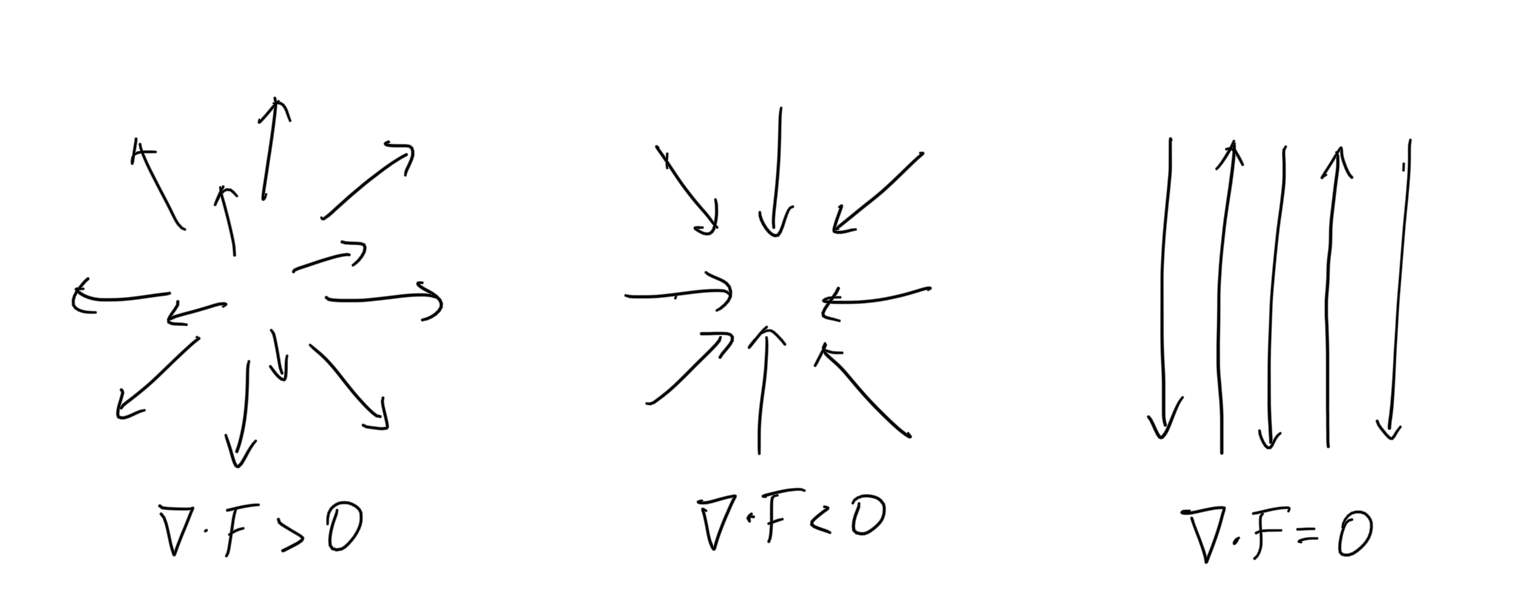
\includegraphics[scale=0.25]{img/Divergence_compared_to_Zero.PNG}
  \end{center}

  \begin{definition}[Divergence]
  The \textbf{divergence} of a vector field $\mathbf{F}: \mathbb{R}^n \longrightarrow \mathbb{R}^n$ is a scalar field defined 
  \[\Div \mathbf{F} \coloneqq \nabla \cdot \mathbf{F} = \begin{pmatrix} \frac{\partial}{\partial x_1} \\ \vdots \\ \frac{\partial}{\partial x_n} \end{pmatrix} \cdot \begin{pmatrix} F_1 \\ \vdots \\ F_n \end{pmatrix} = \sum_i \frac{\partial \mathbf{F}_i}{\partial x_i}\]
  When $n = 1$, $\mathbf{F}$ reduces to a regular function and $\Div \mathbf{F} $ reduces to the ordinary derivative. Some further properties: 
  \begin{enumerate}
      \item By linearity of partials, $\Div$ is also a linear operator. That is, given two vector fields $\mathbf{F}, \mathbf{G}$ and two scalars $\alpha, \beta$, 
      \[\Div (\alpha \mathbf{F} + \beta \mathbf{G}) = \alpha \Div \mathbf{F} + \beta \Div \mathbf{G}\]
      
      \item Divergence satisfies the product rule: Given a vector field $\mathbf{F}: \mathbb{R}^n \longrightarrow \mathbb{R}^n$ and a scalar function $\varphi: \mathbb{R}^n \longrightarrow \mathbb{R}$. 
      \[\nabla \cdot (\varphi \mathbf{F}) = \nabla \varphi \cdot \mathbf{F} + \varphi (\nabla \cdot \mathbf{F})\]
  \end{enumerate}
  \end{definition}

  \begin{example}
  The divergence of the origin in the left graph is clearly negative since the net flow is out of the point, while the divergence of the origin in the right graph is positive since the net fluid flow is in. 

  \begin{center}
  \pgfplotsset{width=7cm,compat=1.16}
  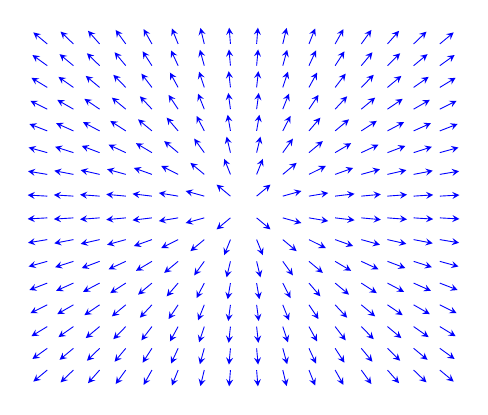
\begin{tikzpicture}[scale=0.8]
  \begin{axis}[view={0}{90}, domain=-4:4, hide axis, zmin=-1, zmax=1, tick label style={font=\tiny}]
  \addplot3 [blue,-stealth,samples=16,
          quiver={
              u={2*x/pow(x^2 + y^2,1/2)},
              v={2*y/pow(x^2 + y^2,1/2)},
              scale arrows=0.2,
          },
      ] {0};
  \end{axis}
  \end{tikzpicture}
  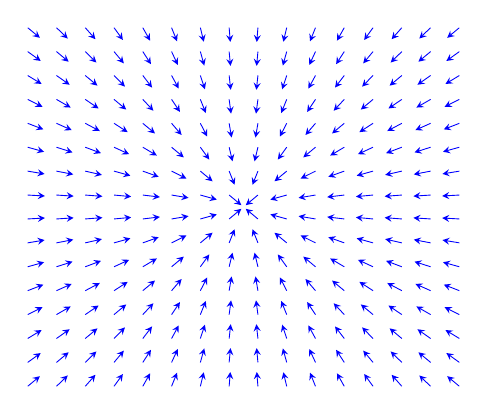
\begin{tikzpicture}[scale=0.8]
  \begin{axis}[view={0}{90}, hide axis, zmin=-1, zmax=1, tick label style={font=\tiny}]
  \addplot3 [blue,-stealth,samples=16,
          quiver={
              u={-2*x/pow(x^2 + y^2,1/2)},
              v={-2*y/pow(x^2 + y^2,1/2)},
              scale arrows=0.2,
          },
      ] {0};
  \end{axis}
  \end{tikzpicture}
  \end{center}
  \end{example}

  \begin{lemma}[Divergence in Cylindrical Coordinates]
  For vector field $F: \mathbb{R}^3 \longrightarrow \mathbb{R}^3$ expressed in cylindrical coordinates as 
  \[F = \begin{pmatrix}
  F_r \\ F_\theta \\ F_z
  \end{pmatrix}\]
  the divergence is
  \[\Div F = \nabla \cdot F = \frac{1}{r} \frac{\partial}{\partial r} \big(r F_r \big) + \frac{1}{r} \frac{\partial F_\theta}{\partial \theta} + \frac{\partial F_z}{\partial z}\]
  Note that the condition of locality is important, since in general a global cylindrical coordinate system would be inconsistent. 
  \end{lemma}

  \begin{lemma}[Divergence in Spherical Coordinates]
  For vector field $F: \mathbb{R}^3 \longrightarrow \mathbb{R}^3$ expressed in spherical coordinates $(r, \theta, \phi)$, the divergence is 
  \[\Div F = \nabla \cdot F = \frac{1}{r^2} \frac{\partial}{\partial r} \big( r^2 F_r) + \frac{1}{r \, \sin{\theta}} \frac{\partial}{\partial \theta} \big( \sin{\theta} F_\theta\big) + \frac{1}{r\, \sin{\theta}} \frac{\partial F_\phi}{\partial \phi}\]
  \end{lemma}

\subsection{Curl}

  Colloquially, the curl is a vector operator that describes the infinitesimal circulation of a vector field in $3$-dimensional Euclidean space, where the curl at each point is represented by a vector whose length and direction denote the magnitude and axis as the maximum circulation. That is, if one drops a twig or a ball with its center of mass at a certain point, the curl measures how much it will spin. In physics, the rotation of a rigid body in 3-dimensions can be described by a vector $\omega$ along the axis of rotation. $\omega$ is called the \textit{angular velocity vector}, with $||\omega||$ denoting the angular speed of the body. The curl of this vector field measured at the center of mass of the body is measured as $2 \omega$. That is, the curl outputs \textit{twice} the angular velocity vector of any rigid body. Note that unlike the gradient and divergence operators, curl does not generalize as simply to other dimensions. 

  \begin{definition}[Curl]
  The \textit{curl} of a 3-dimensional $C^k$ vector field $F: \mathbb{R}^3 \longrightarrow \mathbb{R}^3$ is an operator
  \[\curl: C^k (\mathbb{R}^3; \mathbb{R}^3) \longrightarrow C^{k-1} (\mathbb{R}^3; \mathbb{R}^3)\]
  defined
  \[\curl{F} \equiv \nabla \times F \equiv \begin{pmatrix}
  \frac{\partial}{\partial x} \\ \frac{\partial}{\partial y}\\ \frac{\partial}{\partial z} \end{pmatrix} \equiv \begin{pmatrix}
  \frac{\partial F_3}{\partial y} - \frac{\partial F_2}{\partial z} \\
  \frac{\partial F_1}{\partial z} - \frac{\partial F_3}{\partial x} \\
  \frac{\partial F_2}{\partial x} - \frac{\partial F_1}{\partial y}
  \end{pmatrix}\]
  \end{definition}

  \begin{definition}[Irrotational Vector Fields]
  A vector field $F$ is \textit{irrotational} if 
  \[\curl{F} = \mathbf{0}\]
  Visually, this indicates that there are no "whirlpools" everywhere, meaning that any rigid body placed anywhere, while it may travel along a path, will not rotate around its own axis. 
  \end{definition}

  It has been shown that fluid draining from a tub is usually irrotational except for right at the center, which is surprising since the fluid itself is "rotating" around the drain. 

  \begin{theorem}
  For any $C^2$ vector field $F$, 
  \[\Div{\curl{F}} = \nabla\cdot (\nabla \times F) = 0\]
  That is, the divergence of any curl is 0. 
  \end{theorem}
  \begin{proof}
  Proved by equality of mixed partials. 
  \end{proof}

  \begin{definition}
  The \textit{Laplace operator}, or \textit{Laplacian}, of a function $f: \mathbb{R}^n \longrightarrow \mathbb{R}$ is the divergence of the gradient. 
  \[\nabla^2 f \equiv \nabla \cdot (\nabla f) \equiv \sum_{i=1}^n \frac{\partial^2 f}{\partial x_i^2}\]
  \end{definition}

\subsection{Conservative, Solenoidal Vector Fields}

  \begin{definition}[Conservative Vector Fields]
  A vector field $F: U \subset \mathbb{R}^n \longrightarrow \mathbb{R}^n$ is a \textit{conservative vector field} if and only if there exists a scalar field $f: U \subset \mathbb{R}^n \longrightarrow \mathbb{R}$ such that 
  \[F = \nabla f\]
  on $U$. 
  \end{definition}

  Conservative vector fields appear naturally in mechanics: they are vector fields representing forces of physical systems in which energy is conserved. 

  \begin{theorem}
  Given a $C^2$-function $f: \mathbb{R}^3 \longrightarrow \mathbb{R}$,
  \[\nabla \times ( \nabla f) = 0\]
  That is, the curl of any gradient vector field is the zero vector. 
  \end{theorem}
  \begin{proof}
  $\nabla \times \nabla f$ can be expanded to
  \[\bigg( \frac{\partial^2 f}{\partial y \partial z} - \frac{\partial^2 f}{\partial z \partial y}, \; \frac{\partial^2 f}{\partial z \partial x} - \frac{\partial^2 f}{\partial x \partial z}, \; \frac{\partial^2 f}{\partial x \partial y} - \frac{\partial^2 f}{\partial y \partial x}\bigg) = (0, 0, 0)\]
  by equality of mixed partials. 
  \end{proof}

  \begin{definition}[Solenoidal Vector Fields]
  A \textit{solenoidal, or incompressible, vector field} is a vector field $F: \mathbb{R}^n \longrightarrow \mathbb{R}^n$ such that
  \[\Div F = \nabla \cdot F = 0\]
  at all point in the field. That is, the field has no sources or sinks. 
  \end{definition}

  \begin{example}
  The vector field $F: (x, y) \mapsto (y, -x)$ is solenoidal. 
  \begin{center}
      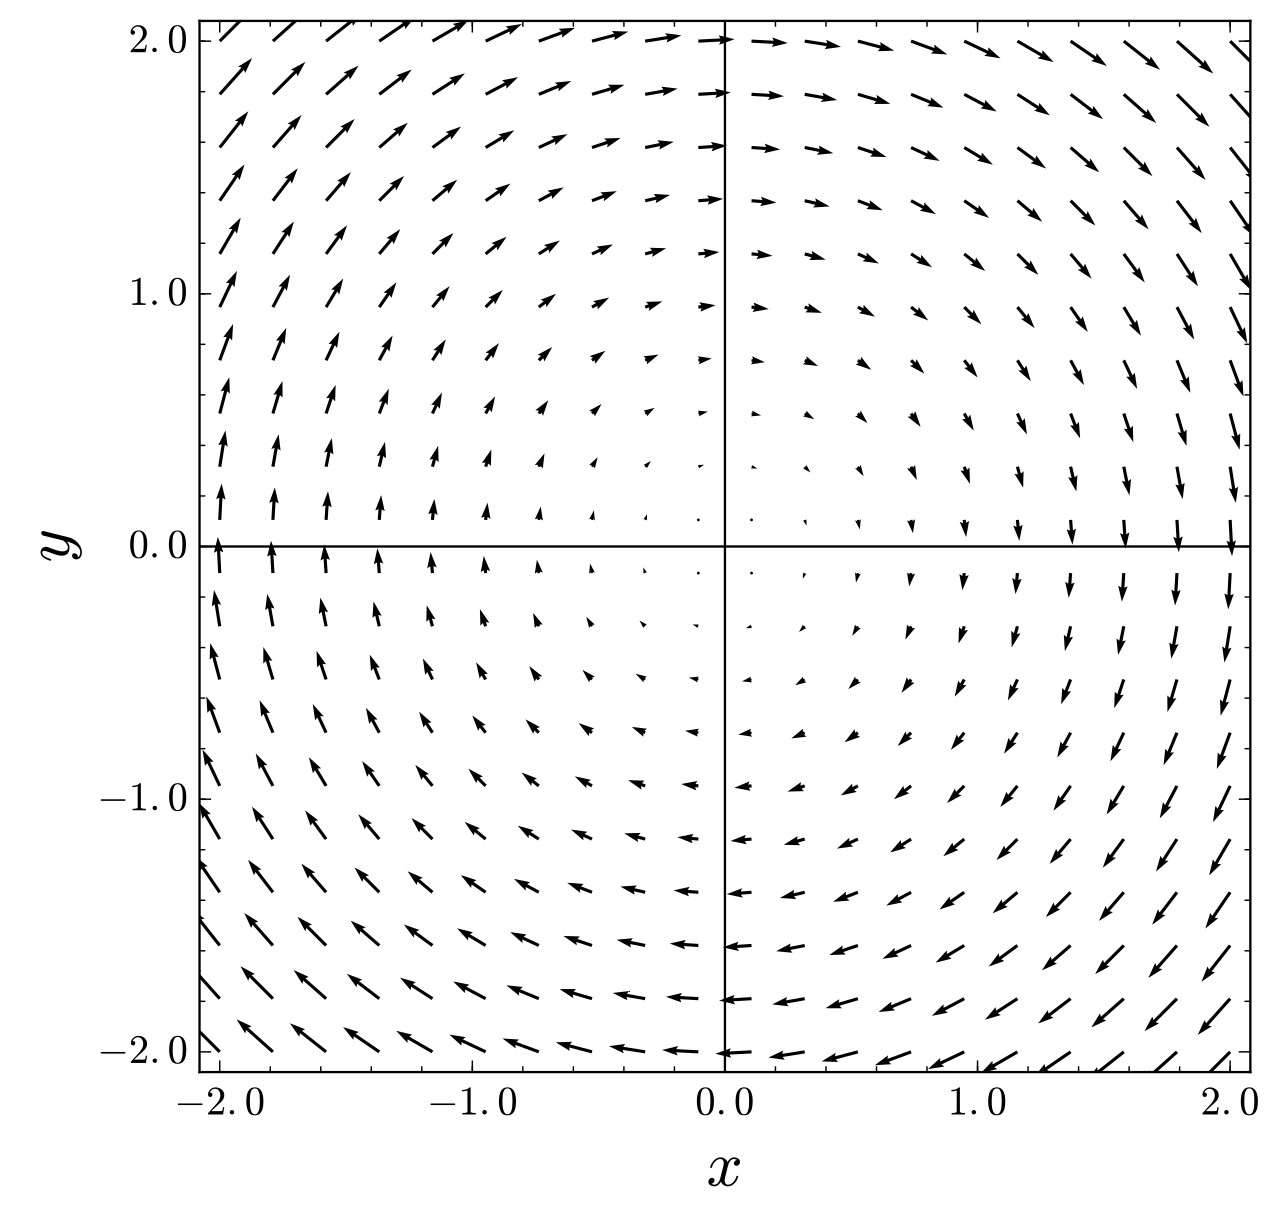
\includegraphics[scale=0.17]{img/Solenoidal_vector_field.png}
  \end{center}
  \end{example}


\section{Riemann and Darboux Integration} 

  We have done integration over closed intervals $[a, b]$. The natural extension is to define integration over \textit{boxes} $B = \prod_i [a_i, b_i]$. Essentially the construction is exactly the same. 

  \begin{definition}[Partition/Mesh]
    Let $B = \prod_i [a_i, b_i] \subset \mathbb{R}^n$ be a box. Then, a \textbf{partition}---or \textbf{mesh}---of $B$ is a finite set of points $P = \{x_{ij}\}_{1 \leq i \leq n, 0 \leq j \leq m_i}$\footnote{Therefore, for each dimension $i$, we want to take the interval $[a_i, b_i]$ and subdivide it into $m_i+1$ subintervals.} s.t. 
    \begin{equation}
      a_i = x_{i, 0} \leq x_{i, 1} \leq x_{i, 2} \leq \ldots \leq x_{i, m_i-1} \leq x_{i, m_i} = b \quad \forall i = 1, \ldots, n
    \end{equation}
    We denote each \textbf{box} within the partition as 
    \begin{equation}
      \Delta_J = \Delta_{j_1, j_2, \ldots, j_n} = \prod_{i} [x_{i, j_k-1}, x_{i, j_k}] \quad \forall j_i = 1, \ldots, m_i
    \end{equation}
    of volume $|\Delta_J| \coloneqq \prod_{i} (x_{i, j_k} - x_{i, j_{k-1}})$. 
  \end{definition}

  This nearly\footnote{since boundaries overlap} partitions $B$ into a grid of $\prod_i m_i$ smaller boxes, and can be seen as a discretization of the integral which we will construcct. 

  \begin{definition}[Riemann Sums with Respect to Partition]
    Let $P$ be a partition of $B \in \mathbb{R}^n$ and let $f: B \subset \mathbb{R}^n \to \mathbb{R}$ be bounded. Then, the \textbf{upper and lower Riemann sums} of $f$ with respect to $P$ are defined 
    \begin{equation}
      U(P, f) \coloneqq \sum_{J} \sup_{x \in \Delta_J} f(x) |\Delta_J|, \qquad L(P, f) \coloneqq \sum_{J} \inf_{x \in \Delta_J} f(x) |\Delta_J|
    \end{equation}

    \begin{figure}[H]
      \centering
      \begin{subfigure}[b]{0.48\textwidth}
        \centering
        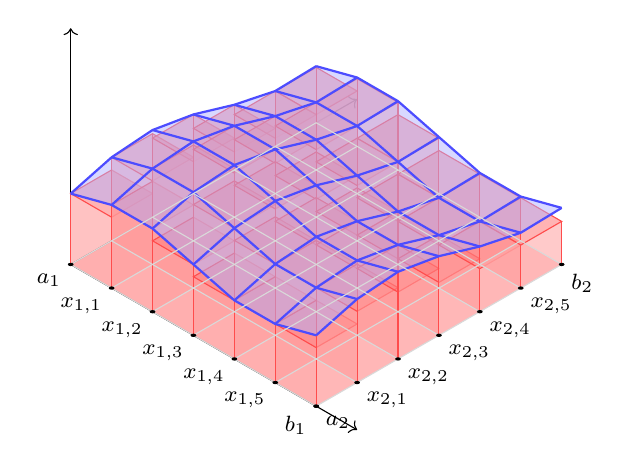
\begin{tikzpicture}[scale=0.6,
          x={(0.866cm,-0.5cm)}, y={(0.866cm,0.5cm)}, z={(0cm,1cm)}]
          
          % Draw axes (without labels)
          \draw[->] (0,0,0) -- (7,0,0);
          \draw[->] (0,0,0) -- (0,7,0);
          \draw[->] (0,0,0) -- (0,0,5);
          
          % Draw rectangular prisms (lower Riemann sum)
          % Using minimum z-value in each cell for lower sum
          \foreach \x in {0,1,2,3,4,5} {
            \foreach \y in {0,1,2,3,4,5} {
              % Calculate heights at four corners of the cell
              \pgfmathsetmacro{\zaa}{1.5 + 0.3*sin(\x*60) + 0.35*sin(\y*50)}
              \pgfmathsetmacro{\zba}{1.5 + 0.3*sin((\x+1)*60) + 0.35*sin(\y*50)}
              \pgfmathsetmacro{\zbb}{1.5 + 0.3*sin((\x+1)*60) + 0.35*sin((\y+1)*50)}
              \pgfmathsetmacro{\zab}{1.5 + 0.3*sin(\x*60) + 0.35*sin((\y+1)*50)}
              
              % Find minimum height (lower Riemann sum)
              \pgfmathsetmacro{\zmin}{min(\zaa,min(\zba,min(\zbb,\zab)))}
              
              % Bottom face (on xy-plane)
              \fill[red!30, opacity=0.6] (\x,\y,0) -- (\x+1,\y,0) -- (\x+1,\y+1,0) -- (\x,\y+1,0) -- cycle;
              
              % Front face
              \fill[red!40, opacity=0.6] (\x,\y,0) -- (\x+1,\y,0) -- (\x+1,\y,\zmin) -- (\x,\y,\zmin) -- cycle;
              
              % Right face
              \fill[red!35, opacity=0.6] (\x+1,\y,0) -- (\x+1,\y+1,0) -- (\x+1,\y+1,\zmin) -- (\x+1,\y,\zmin) -- cycle;
              
              % Top face
              \fill[red!50, opacity=0.6] (\x,\y,\zmin) -- (\x+1,\y,\zmin) -- (\x+1,\y+1,\zmin) -- (\x,\y+1,\zmin) -- cycle;
              
              % Draw edges
              \draw[red!70] (\x,\y,0) -- (\x,\y,\zmin);
              \draw[red!70] (\x+1,\y,0) -- (\x+1,\y,\zmin);
              \draw[red!70] (\x+1,\y+1,0) -- (\x+1,\y+1,\zmin);
              \draw[red!70] (\x,\y+1,0) -- (\x,\y+1,\zmin);
              \draw[red!70] (\x,\y,\zmin) -- (\x+1,\y,\zmin) -- (\x+1,\y+1,\zmin) -- (\x,\y+1,\zmin) -- cycle;
            }
          }
          
          % Draw surface patches first (back to front for proper layering)
          \foreach \ystart/\yend in {0/1, 1/2, 2/3, 3/4, 4/5, 5/6} {
            \foreach \xstart/\xend in {0/1, 1/2, 2/3, 3/4, 4/5, 5/6} {
              \pgfmathsetmacro{\zaa}{1.5 + 0.3*sin(\xstart*60) + 0.35*sin(\ystart*50)}
              \pgfmathsetmacro{\zba}{1.5 + 0.3*sin(\xend*60) + 0.35*sin(\ystart*50)}
              \pgfmathsetmacro{\zbb}{1.5 + 0.3*sin(\xend*60) + 0.35*sin(\yend*50)}
              \pgfmathsetmacro{\zab}{1.5 + 0.3*sin(\xstart*60) + 0.35*sin(\yend*50)}
              
              \fill[blue!30, opacity=0.5] 
                (\xstart,\ystart,\zaa) --
                (\xend,\ystart,\zba) --
                (\xend,\yend,\zbb) --
                (\xstart,\yend,\zab) -- cycle;
            }
          }
          
          % Draw grid lines on surface
          % Lines parallel to x-axis
          \foreach \y in {0,1,2,3,4,5,6} {
            \draw[blue!70, thick] 
              (0,\y,{1.5 + 0.35*sin(\y*50)}) 
              \foreach \x in {1,2,3,4,5,6} {
                -- (\x,\y,{1.5 + 0.3*sin(\x*60) + 0.35*sin(\y*50)})
              };
          }
          
          % Lines parallel to y-axis
          \foreach \x in {0,1,2,3,4,5,6} {
            \draw[blue!70, thick] 
              (\x,0,{1.5 + 0.3*sin(\x*60)}) 
              \foreach \y in {1,2,3,4,5,6} {
                -- (\x,\y,{1.5 + 0.3*sin(\x*60) + 0.35*sin(\y*50)})
              };
          }
          
          % Base grid
          \foreach \x in {0,1,2,3,4,5,6} {
            \draw[gray!30, thin] (\x,0,0) -- (\x,6,0);
            \draw[gray!30, thin] (0,\x,0) -- (6,\x,0);
          }
          
          % X-axis tick labels (back axis)
          \foreach \x/\label in {0/a_1, 1/x_{1,1}, 2/x_{1,2}, 3/x_{1,3}, 4/x_{1,4}, 5/x_{1,5}, 6/b_1} {
            \fill (\x,0,0) circle (0.05);
            \node[below left, font=\footnotesize] at (\x,0,0) {$\label$};
          }
          
          % Y-axis tick labels (front axis at x=6)
          \foreach \y/\label in {0/a_2, 1/x_{2,1}, 2/x_{2,2}, 3/x_{2,3}, 4/x_{2,4}, 5/x_{2,5}, 6/b_2} {
            \fill (6,\y,0) circle (0.05);
            \node[below right, font=\footnotesize] at (6,\y,0) {$\label$};
          }
        \end{tikzpicture}
        \caption{Lower Riemann sum.}
        \label{fig:lower_riemann_sum}
      \end{subfigure}
      \hfill 
      \begin{subfigure}[b]{0.48\textwidth}
        \centering
        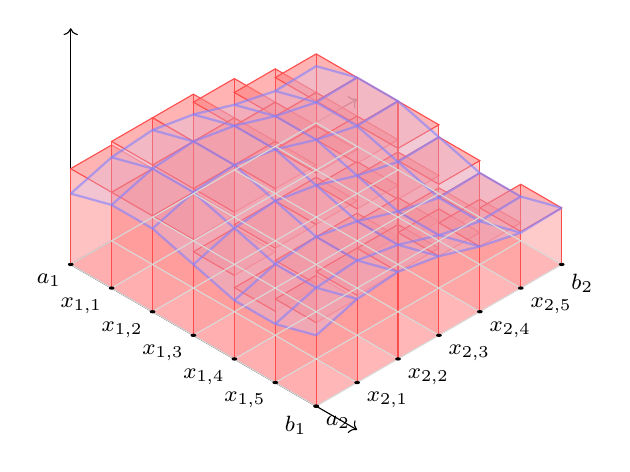
\begin{tikzpicture}[scale=0.6,
          x={(0.866cm,-0.5cm)}, y={(0.866cm,0.5cm)}, z={(0cm,1cm)}]
          
          % Draw axes (without labels)
          \draw[->] (0,0,0) -- (7,0,0);
          \draw[->] (0,0,0) -- (0,7,0);
          \draw[->] (0,0,0) -- (0,0,5);
          
          % Draw rectangular prisms (upper Riemann sum)
          % Using maximum z-value in each cell for upper sum
          \foreach \x in {0,1,2,3,4,5} {
            \foreach \y in {0,1,2,3,4,5} {
              % Calculate heights at four corners of the cell
              \pgfmathsetmacro{\zaa}{1.5 + 0.3*sin(\x*60) + 0.35*sin(\y*50)}
              \pgfmathsetmacro{\zba}{1.5 + 0.3*sin((\x+1)*60) + 0.35*sin(\y*50)}
              \pgfmathsetmacro{\zbb}{1.5 + 0.3*sin((\x+1)*60) + 0.35*sin((\y+1)*50)}
              \pgfmathsetmacro{\zab}{1.5 + 0.3*sin(\x*60) + 0.35*sin((\y+1)*50)}
              
              % Find maximum height (upper Riemann sum)
              \pgfmathsetmacro{\zmax}{max(\zaa,max(\zba,max(\zbb,\zab)))}
              
              % Bottom face (on xy-plane)
              \fill[red!30, opacity=0.6] (\x,\y,0) -- (\x+1,\y,0) -- (\x+1,\y+1,0) -- (\x,\y+1,0) -- cycle;
              
              % Front face
              \fill[red!40, opacity=0.6] (\x,\y,0) -- (\x+1,\y,0) -- (\x+1,\y,\zmax) -- (\x,\y,\zmax) -- cycle;
              
              % Right face
              \fill[red!35, opacity=0.6] (\x+1,\y,0) -- (\x+1,\y+1,0) -- (\x+1,\y+1,\zmax) -- (\x+1,\y,\zmax) -- cycle;
              
              % Top face
              \fill[red!50, opacity=0.6] (\x,\y,\zmax) -- (\x+1,\y,\zmax) -- (\x+1,\y+1,\zmax) -- (\x,\y+1,\zmax) -- cycle;
              
              % Draw edges
              \draw[red!70] (\x,\y,0) -- (\x,\y,\zmax);
              \draw[red!70] (\x+1,\y,0) -- (\x+1,\y,\zmax);
              \draw[red!70] (\x+1,\y+1,0) -- (\x+1,\y+1,\zmax);
              \draw[red!70] (\x,\y+1,0) -- (\x,\y+1,\zmax);
              \draw[red!70] (\x,\y,\zmax) -- (\x+1,\y,\zmax) -- (\x+1,\y+1,\zmax) -- (\x,\y+1,\zmax) -- cycle;
            }
          }
          
          % Draw surface patches with lighter opacity
          \foreach \ystart/\yend in {0/1, 1/2, 2/3, 3/4, 4/5, 5/6} {
            \foreach \xstart/\xend in {0/1, 1/2, 2/3, 3/4, 4/5, 5/6} {
              \pgfmathsetmacro{\zaa}{1.5 + 0.3*sin(\xstart*60) + 0.35*sin(\ystart*50)}
              \pgfmathsetmacro{\zba}{1.5 + 0.3*sin(\xend*60) + 0.35*sin(\ystart*50)}
              \pgfmathsetmacro{\zbb}{1.5 + 0.3*sin(\xend*60) + 0.35*sin(\yend*50)}
              \pgfmathsetmacro{\zab}{1.5 + 0.3*sin(\xstart*60) + 0.35*sin(\yend*50)}
              
              \fill[blue!20, opacity=0.25] 
                (\xstart,\ystart,\zaa) --
                (\xend,\ystart,\zba) --
                (\xend,\yend,\zbb) --
                (\xstart,\yend,\zab) -- cycle;
            }
          }
          
          % Draw grid lines on surface (lighter)
          % Lines parallel to x-axis
          \foreach \y in {0,1,2,3,4,5,6} {
            \draw[blue!50, thick, opacity=0.6] 
              (0,\y,{1.5 + 0.35*sin(\y*50)}) 
              \foreach \x in {1,2,3,4,5,6} {
                -- (\x,\y,{1.5 + 0.3*sin(\x*60) + 0.35*sin(\y*50)})
              };
          }
          
          % Lines parallel to y-axis
          \foreach \x in {0,1,2,3,4,5,6} {
            \draw[blue!50, thick, opacity=0.6] 
              (\x,0,{1.5 + 0.3*sin(\x*60)}) 
              \foreach \y in {1,2,3,4,5,6} {
                -- (\x,\y,{1.5 + 0.3*sin(\x*60) + 0.35*sin(\y*50)})
              };
          }
          
          % Base grid
          \foreach \x in {0,1,2,3,4,5,6} {
            \draw[gray!30, thin] (\x,0,0) -- (\x,6,0);
            \draw[gray!30, thin] (0,\x,0) -- (6,\x,0);
          }
          
          % X-axis tick labels (back axis)
          \foreach \x/\label in {0/a_1, 1/x_{1,1}, 2/x_{1,2}, 3/x_{1,3}, 4/x_{1,4}, 5/x_{1,5}, 6/b_1} {
            \fill (\x,0,0) circle (0.05);
            \node[below left, font=\footnotesize] at (\x,0,0) {$\label$};
          }
          
          % Y-axis tick labels (front axis at x=6)
          \foreach \y/\label in {0/a_2, 1/x_{2,1}, 2/x_{2,2}, 3/x_{2,3}, 4/x_{2,4}, 5/x_{2,5}, 6/b_2} {
            \fill (6,\y,0) circle (0.05);
            \node[below right, font=\footnotesize] at (6,\y,0) {$\label$};
          }
        \end{tikzpicture}
        \caption{Upper Riemann sum.}
        \label{fig:upper_riemann_rum}
      \end{subfigure}
      \caption{}
    \end{figure}
  \end{definition}

  \begin{definition}[Riemann Integral]
    Given that $f: B \subset \mathbb{R}^n \to \mathbb{R}$ is bounded, the \textbf{upper and lower Riemann integrals} of $f$ are defined 
    \begin{equation}
      \overline{\int_B} f(x) \,dx \coloneqq \inf_P U(P, f), \qquad \underline{\int_B} f(x) \,dx \coloneqq \sup_P L(P, f) 
    \end{equation}
    If the upper and lower Riemann integrals are equal, then the \textbf{Riemann integral} of $f$ 
    \begin{equation}
      \int_B f(x) \,dx 
    \end{equation}
    is defined as such. Furthermore, $f$ is said to be \textbf{Riemann integrable} over $B$. 
  \end{definition} 

\subsection{Conditions for Integrability} 

  \begin{theorem}[]
    $f: B \subset \mathbb{R}^n \to \mathbb{R}$ continuous means $f$ is integrable over $B$. 
  \end{theorem}

  However, there are some functions with discontinuities that are in fact integrable. 
  \begin{enumerate}
    \item Given that there is a subset $N$ in $B$ with volume $0$ over which $f$ is not defined, we can integrate over $B \setminus N$. In the one and two dimensional cases, 
    \[\int_{B \setminus N} f(x) dx \text{ and } \iint_{B\setminus N} f(x) dA\]
    are well-defined. Visually, 
    \begin{center}
      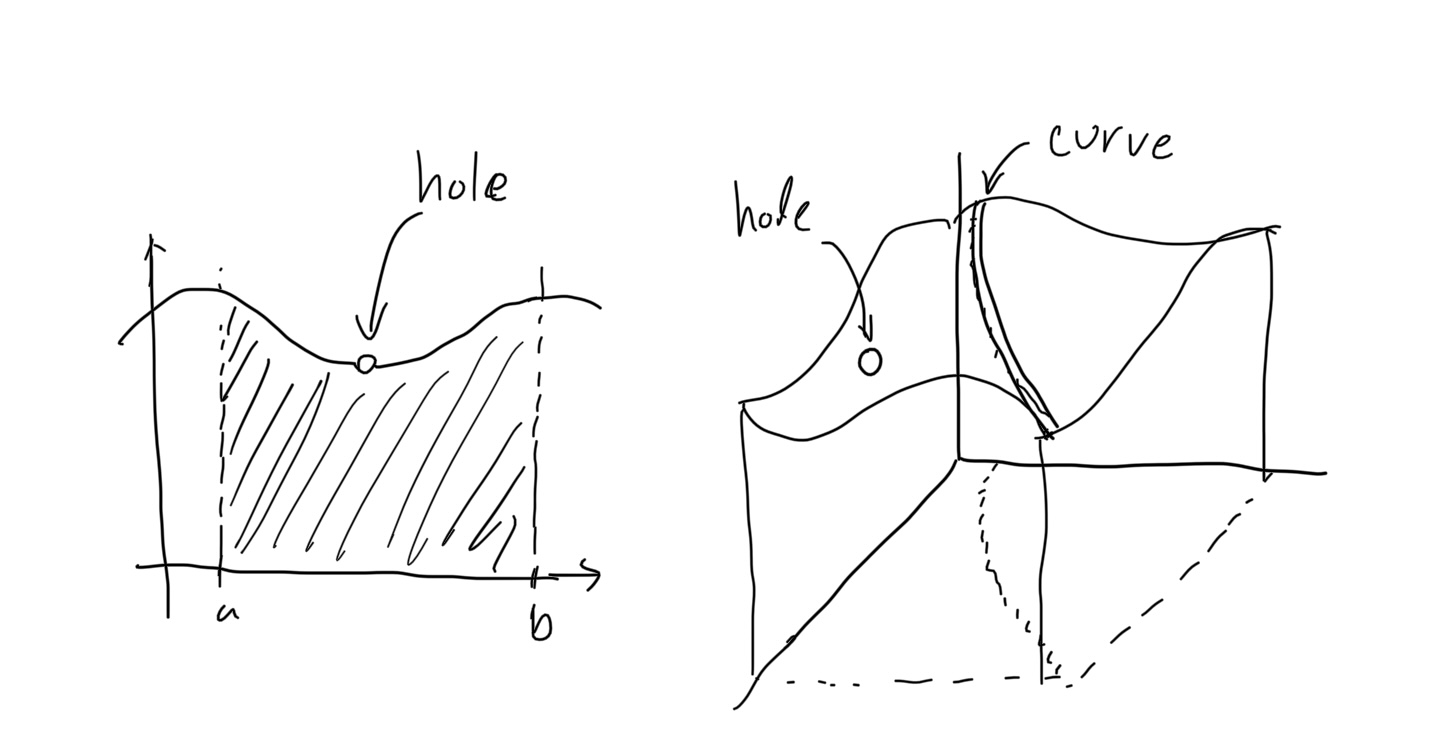
\includegraphics[scale=0.2]{img/Integrable_Hole_Function.jpg}
    \end{center}
    \item The function is defined for all values in the region, but there is a jump in the value of the function. 
    \begin{center}
      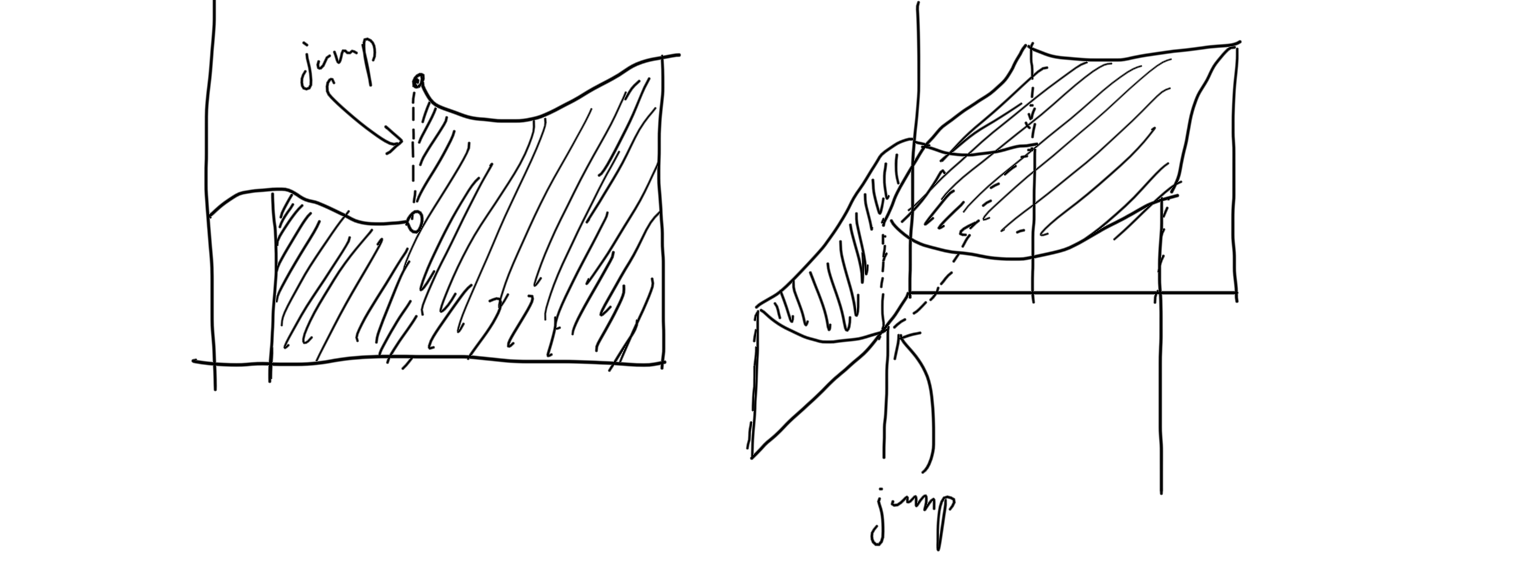
\includegraphics[scale=0.23]{img/Integrable_Jump_Function.PNG}
    \end{center}
  \end{enumerate}
  Informally, if we can visualize the Riemann sum converging to a well-defined area as the rectangles get thinner and thinner, then a discontinuous function is integrable. Indeed, all continuous functions (over a bounded set) are integrable since their Riemann sums are well defined. 


\subsection{Iterated Integrals and Fubini's Theorem} 

  The construction of the integral is one step, but we should know how to practically compute such an integral. We can do this by recursively ``reducing'' the dimension of the region of the integral until we can work with one dimension. This is known as \textit{Cavalieri's principle}: Let $S$ be a bounded $n$-dimensional solid in $\mathbb{R}^n$. Define an $n-1$ subspace $P$ in $\mathbb{R}^n$ and given the quotient space $\mathbb{R}^n / P$ with elements $P_x$, let 
  \begin{equation}
    S \subset \bigcup_{a \leq x \leq b} P_x
  \end{equation}
  That is, $S$ is "in between" affine subspaces $P_a$ and $P_b$. Given the cross section of $S$ with $P_x$, defined $P_x \cap S$, denote the integral of this cross section as $A(x)$. Then, colloquially, the volume of $S$ can be represented as the integral $\int_a^b A(x)\,dx$. This idea basically says that the volume of $S$ is the sum of the areas of its infinitesimal cross sections. 

  \begin{figure}[H]
    \centering 
    
\includegraphics[scale=0.27]{img/Cavalieri_Principle.PNG}
    \caption{Visual of Cavalieri's principle.} 
    \label{fig:cavalieri}
  \end{figure}

  Given a solid $S \subset \mathbb{R}^n$, it is easy to see that no matter what subspace $P$ we choose–that is, no matter what orientation we choose to "cut" the solid– the sum of all of its cross sections should be equal to the true volume of $S$. In the case when $S$ is a box in $\mathbb{R}^n$, Fubini's theorem states that whether we cut $S$ up along the $x_1$-axis, $x_2$-axis, ..., or the $x_n$-axis, the symmetry in volume is always preserved. This theorem is really just a specific case of this general symmetry in volume. 

  \begin{theorem}[Fubini's Theorem]
    Given a function $f: \mathbb{R}^n \longrightarrow \mathbb{R}$, let 
    \[B \equiv \prod_{i=1}^n [\alpha_i, \beta_i]\]
    and let 
    $p$ be any permutation of the elements $\{x_1, x_2, ..., x_n\}$. Then 
    \begin{align*}
        \int_B f \; d V & = \int_{\alpha_n}^{\beta_n} ... \int_{\alpha_1}^{\beta_1} f(x_1,x_2,...,x_n) \; d x_1 ... d x_n \\
        & = \int_{p(\alpha_n)}^{p(\beta_n)} ... \int_{p(\alpha_1)}^{p(\beta_1)} f(x_1,x_2, ..., x_n) \; d p(x_1) ... d p(x_n) 
    \end{align*}
    In the two dimensional case, we have
    \begin{align*}
        \iint_B f \; d A & = \int_c^d \int_a^b f(x, y) \; d x \, d y = \int_a^b \int_c^d f(x, y) \; d y \, d x 
    \end{align*}
    \begin{center}
        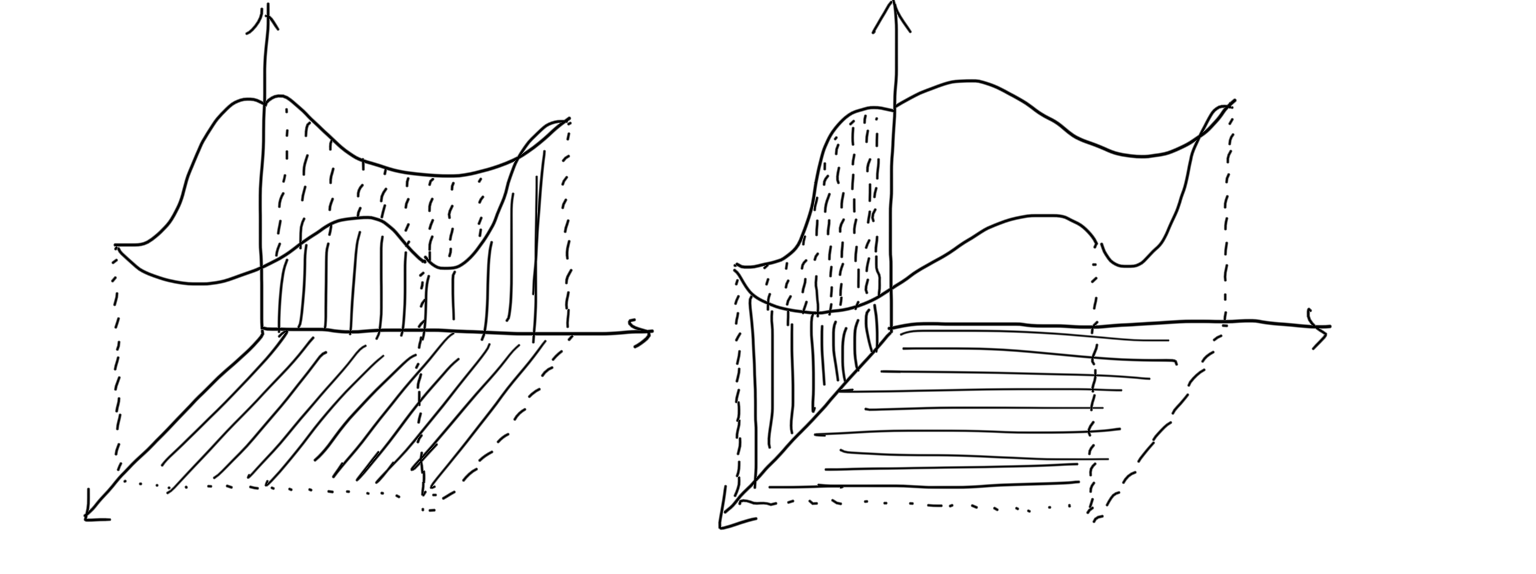
\includegraphics[scale=0.27]{img/Fubini_Theorem.PNG}
    \end{center}
    In the three dimensional case, we have
    \begin{align*}
        \iiint_B f \; d V & 
        = \int_e^f \int_c^d \int_a^b f(x, y, z) \; d x \, d y \, d z = \int_e^f \int_a^b \int_c^d f(x, y, z) \; d y \, d x \, d z \\
        & = \int_c^d \int_a^b \int_e^f f(x, y, z) \; d z \, d x \, d y = \int_c^d \int_e^f \int_a^b f(x, y, z) \; d x \, d z \, d y \\
        & = \int_a^b \int_e^f \int_c^d f(x, y, z) \; d y \, d z \, d x = \int_a^b \int_c^d \int_e^f f(x, y, z) \; d z \, d y \, d x 
    \end{align*}
  \end{theorem}

  Computation of these integrals is simple. You do the innermost integral first with respect to the corresponding variable, while treating the rest of the variables constant. Evaluating each integral outputs a formula for a higher dimensional cross section of the solid $S$. It is clear that computing iterated integrals is really just doing Cavalieri's principle repeatedly. 

\subsection{Integration over Regions between Curves} 

  \begin{definition}[Simple Regions w.r.t. a Variable]
    A bounded region $D$ in $\mathbb{R}^n$ is said to be $x_i$-simple if it is bounded by the graphs of two continuous functions $u_1, u_2: \mathbb{R}^{n-1} \longrightarrow \mathbb{R}$ of the variables 
    \[x_1, x_2, ..., x_{i-1}, x_{i+1}, ..., x_n\]
    That is, $D$ can be expressed in the form 
    \[\{ x \in \mathbb{R}^n \; | \; u_1 (x_1,..., x_{i-1}, x_{i+1}, ... , x_n) \leq x_i \leq u_2 (x_1, ..., x_{i-1}, x_{i+1}, ..., x_n)\}\]
    If a region is simple in all of its variables, it is simply called \textit{simple}. Note that $n$-dimensional boxes are simple regions. 
  \end{definition}

  \begin{example}
    In $\mathbb{R}^2$, the region on the left graph is an $y$-simple region and the region on the right is a $x$-simple region. 
    \begin{center}
    \begin{tikzpicture}[scale=0.8]
      \draw[<->] (-1,0)--(5,0);
      \draw[<->] (0,-1)--(0,5);
      \draw[<->] (6,0)--(12,0);
      \draw[<->] (7,-1)--(7,5);
      \draw plot [smooth] coordinates {(0.6, 1.2) (1,1) (2,1.4) (3,1.3) (4,1.5) (4.3,1.7)};
      \draw plot [smooth] coordinates {(0.6, 3.9) (1,4.1) (2,4) (3,4.3) (4,4.2) (4.3,4.1)};
      \draw[dashed] (0.6,1.2)--(0.6,3.9);
      \draw[dashed] (4.3,1.7)--(4.3,4.1);
      \draw plot [smooth] coordinates {(8.2,0.6) (8,1) (8.4,2) (8.3,3) (8.5,4) (8.7,4.3)};
      \draw plot [smooth] coordinates {(10.9,0.6) (11.1,1) (11,2) (11.3,3) (11.2,4) (11.1,4.3)};
      \draw[dashed] (8.2,0.6)--(10.9,0.6);
      \draw[dashed] (8.7,4.3)--(11.1,4.3);
      \node[below] at (4.8,0) {$x$};
      \node[below] at (11.8,0) {$x$};
      \node[left] at (0,4.8) {$y$};
      \node[left] at (7,4.8) {$y$};
      \node[above] at (3,4.2) {$u_1$};
      \node[above] at (3,1.3) {$u_2$};
      \node[left] at (8.3, 3) {$v_1$};
      \node[right] at (11.3, 3) {$v_2$};
      \draw[fill] (0.6,0) circle (0.05);
      \node[below] at (0.6,0) {$a$};
      \draw[fill] (4.3,0) circle (0.05);
      \node[below left] at (4.3,0) {$b$};
      \draw[fill] (7,0.6) circle (0.05);
      \draw[fill] (7,4.3) circle (0.05);
      \node[left] at (7,0.6) {$c$};
      \node[left] at (7,4.3) {$d$};
    \end{tikzpicture}
    \end{center}
  \end{example}

  We now describe the method of calculating double integrals over elementary regions. 
  \begin{theorem}
  The double integral over a $y$-simple region $D$ bounded by functions $u_1$ and $u_2$ in $\mathbb{R}^2$ and the $x$-values $a$ and $b$ (as shown in the left graph of example 2.1) is
  \[\iint_D f(x, y) = \int_a^b \int_{u_2 (x)}^{u_1 (x)} f(x, y) \, dy \, dx\]
  The double integral over an $x$-simple region $D$ bounded by functions $v_1$ and $v_2$ in $\mathbb{R}^2$ and the $y$-values $c$ and $d$ (shown in the right of graph of example 2.1) is 
  \[\iint_D f(x, y) = \int_c^d \int_{v_2 (y)}^{v_1 (y)} f(x, y) \, dx \, dy\]
  \end{theorem}

  \begin{example}
  Integrating $f(x, y)$ over the unit disk would have the form
  \[\int_{-1}^1 \int_{-\sqrt{1-x^2}}^{\sqrt{1-x^2}} f(x,y) \, dy\, dx \text{ or } \int_{-1}^1 \int_{-\sqrt{1-y^2}}^{\sqrt{1-y^2}} f(x,y) \, dx\, dy \]
  Note that the unit disk is both $x$ and $y$ simple. 
  \end{example}

\subsection{Change of Basis}

  Sometimes, integrating a region over a different basis would make the integral computation much more simpler. In this case, we may be able to transform more complicated regions into elementary regions. We first introduce a change of basis in 2 dimensions and then generalize it into higher dimensions. 
  
  Let $\mathbb{R}^2$ have the standard orthonomal basis $e_1, e_2$, commonly known as the $x, y$ basis. Now, let us construct new basis vectors of $\mathbb{R}^2$, denoted $f_1, f_2$ such that $f_1, f_2$ are functions of $e_1, e_2$. Since they are both bases that span $\mathbb{R}^2$, we can equally represent $e_1, e_2$ as functions of $f_1, f_2$. 
  \begin{align*}
      &e_1 = g(f_1, f_2)\\
      &e_2 = h(f_1, f_2) 
  \end{align*}
  Note that this change of basis does not necessarily have to be linear, as in the context of passive transformation in linear algebra. Then, every point $(x,y)$ in the $(e_1, e_2)$-basis can be rewritten as
  \begin{align*}
      (x, y) & = x e_1 + y e_2 \\
      & = x \, g(f_1, f_2) + y \, h(f_1, f_2) \\
      & = u f_1 + v f_2
  \end{align*}
  Note that it is customary to denote $x, y$ as the coefficients in the $e_1, e_2$ basis and $u, v$ as the coefficients in the new $f_1, f_2$ basis. This way, we can not only write $e_1$ and $e_2$ as functions of $f_1$ and $f_2$, but we can also write the coefficents $x, y$ as functions of the coeffiecents $u, v$! That is, 
  \begin{align*}
      & x = x(u, v) \\
      & y = y(u, v)
  \end{align*}
  which is really just a function 
  \[B: \mathbb{R}^2 \longrightarrow \mathbb{R}^2, \;\; B(u, v) = \begin{pmatrix} x(u, v) \\ y(u, v) \end{pmatrix}\]
  Notice that $B$ changes the $u, v$ coordinates to the $x, y$ coordinates, and $B^{-1}$ changes the $x, y$ coordinates to the $u, v$ coordinates. 
  \[B^{-1}: \mathbb{R}^2 \longrightarrow \mathbb{R}^2, \;\; B^{-1} (x, y) = \begin{pmatrix} u (x, y) \\ v (x, y) \end{pmatrix}\]
  Note that these coefficients actually change \textit{contravariantly}, that is, they change inversely with respect to how the basis vectors are changed. In vector calculus, it is conventional to represent a change of basis with functions that relate the coefficients $x, y$ with $u, v$, rather than the bases $f_1, f_2$ with $e_1, e_2$. 

  \begin{theorem}[Integration over Change of Bases in $\mathbb{R}^2$]
  Let $\mathbb{R}^2$ have the standard orthonomal basis $e_1, e_2$. Now, let us construct new basis vectors of $\mathbb{R}^2$, denoted $f_1, f_2$ such that the coefficients of the vectors in $\mathbb{R}^2$ are related by the change of basis function 
  \[B = \begin{pmatrix} x \\ y \end{pmatrix} \implies B(u, v) = \begin{pmatrix} x(u, v) \\ y(u, v) \end{pmatrix}\]
  Given region $D \subset \mathbb{R}^2$ and $S = B(D)$ is the region transformed by $B$, the integral of function $f(x, y)$ over region $D$ can be expressed as 
  \[\iint_D f(x, y) \, dA = \iint_S f \big( x(u, v), y(u, v) \big) \, \big| J B(u, v) \big| \, d \bar{A}\]
  where $\big| J B(u, v) \big|$ is the determinant of the Jacobian matrix of $B$. Expanding the Facobian determinant gives
  \[\big| J B(u, v) \big| = \frac{\partial x}{\partial u} \frac{\partial y}{\partial v} - \frac{\partial x}{\partial v} \frac{\partial y}{\partial u}\]
  \end{theorem}

  \begin{theorem}[Integration over Change of Bases in $\mathbb{R}^3$]
  Given that we have the change of basis function 
  \[B: \mathbb{R}^3 \longrightarrow \mathbb{R}^3, \;\;\; B(u, v, w) = \begin{pmatrix} x(u, v, w) \\ y(u, v, w) \\ z(u, v, w) \end{pmatrix}\]
  a region $D \in \mathbb{R}^3$ and $S = B(D)$, the region transformed by $B$, the integral of $f(x, y, z)$ over region $D$ can be expressed as 
  \[\iiint_D f(x, y, z)\, dV = \iiint_S f\big( x(u, v, w), y(u, v ,w), z(u, v, w) \big) \big| J B (u, v, w)\big| \, d \bar{V}\]
  where $\big| J B (u, v, w)\big|$ is the Jacobian determinant of $B$. 
  \end{theorem}

  \begin{example}
  Given a real-valued function $f$ defined over the region $D \subset \mathbb{R}^2$, we can perform a change of basis of the $x, y$ coordinates into polar ones within a new region $S$. The change of basis 
  \begin{align*}
      & x = r \cos{\theta} \\
      & y = r \sin{\theta} 
  \end{align*}
  \begin{center}
  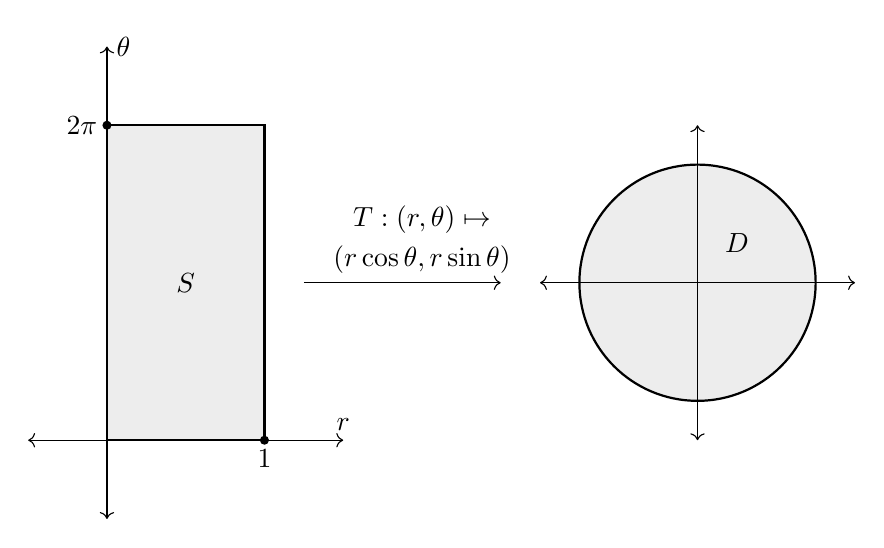
\begin{tikzpicture}
      \draw[thick, fill=lightgray] (7.5,2) circle (1.5);
      \draw[<->] (-1,0)--(3,0);
      \draw[<->] (0,-1)--(0,5);
      \draw[thick, fill=lightgray] (0,0) rectangle (2,4);
      \node at (1,2) {$S$};
      \draw[fill] (0,4) circle (0.05);
      \draw[fill] (2,0) circle (0.05);
      \node[below] at (2,0) {$1$};
      \node[left] at (0,4) {$2 \pi$};
      \node[above] at (3,0) {$r$};
      \node[right] at (0,5) {$\theta$};
      \draw[->] (2.5, 2)--(5,2);
      \node[above] at (4,2.5) {$T: (r, \theta) \mapsto$};
      \node[above] at (4,2) {$ (r \cos{\theta}, r \sin{\theta})$};
      \draw[<->] (5.5,2)--(9.5,2);
      \draw[<->] (7.5,0)--(7.5,4);
      \node at (8,2.5) {$D$};
  \end{tikzpicture}  
  \end{center}
  \end{example}

  \begin{theorem}[Integration over Change of Bases in $\mathbb{R}^n$]
  Let $\mathbb{R}^n$ have the standard orthonormal basis $e_1, e_2, ..., e_n$, and let us construct a new basis $f_1, f_2, ..., f_n$ such that the coefficients of the vectors in $\mathbb{R}^n$ are related with the functions
  \[B: \mathbb{R}^n \longrightarrow \mathbb{R}^n, \;\;\;\; B(u_1, u_2, \ldots, u_n) = \begin{pmatrix}
  x_1 (u_1, \ldots, u_n) \\x_2 (u_1, \ldots, u_n) \\ \vdots \\ x_n (u_1, \ldots, u_n)
  \end{pmatrix}\]
  Given that the region $D \subset \mathbb{R}^n$ is transformed into a new region $S = B(D) \subset \mathbb{R}^n$ under this basis transformation, the integral of function $f(x_1, \ldots, x_n)$ over region $D$ can be expressed as 
  \[\int_D f(x) \, dH = \int_S f \big( x_1(u), x_2(u), ..., x_n (u) \big) \big| J B(u_1, \ldots, u_n)\big| \, d \bar{H}\]
  where the integral on both the left and right hand side represents integration over an $n$-dimensional region, $x$ represents the $n$-tuple $(x_1, \ldots, x_n)$, $u$ represents the $n$-tuple $(u_1, \ldots, u_n)$, and $\big| J B(u_1, \ldots, u_n)\big|$ represents the Jacobian determinant of function $B$. 
  \end{theorem}

  We now describe some common change of basis formulas for polar, cylindrical, and spherical coordinates. 

  \begin{theorem}[Integration in Polar Coordinates]
  \[\iint_{D} f(x, y) \, dx \,dy = \iint_S f(r \cos{\theta}, r \sin{\theta}) r \, dr \, d\theta\]
  \end{theorem}

  \begin{definition}[Cylindrical, Spherical Coordinates]
  In $\mathbb{R}^3$, \textit{cylindrical coordinates} have the following relation to rectangular coordinates. 
  \begin{align*}
      & x = r \cos{\theta} \\
      & y = r \sin{\theta} \\
      & z = z
  \end{align*}
  In $\mathbb{R}^3$, \textit{spherical coordinates} have the following relation to rectangular coordinates. 
  \begin{align*}
      & x = \rho \sin{\phi} \cos{\theta} \\
      & y = \rho \sin{\phi} \sin{\theta} \\
      & z = \rho \cos{\phi}
  \end{align*}
  \end{definition}

  \begin{corollary}[Integration in Cylindrical Coordinates]
  \[\iiint_D f(x, y, z) \, dx \, dy \, dz = \iiint_S f( r \cos{\theta}, r \sin{\theta}, z) r \, dr \, d\theta \, dz\]
  \end{corollary}

  \begin{corollary}[Integration in Spherical Coordinates]
  \[\iiint_D f(x, y, z) \,dx\,dy\,dz = \iiint_S f(\rho \sin{\phi} \cos{\theta}, \rho \sin{\phi} \sin{\theta}, \rho \cos{\phi}) \rho^2 \sin{\theta} \, d\rho \, d\theta \, d\phi\]
  \end{corollary}

  \begin{example}[Gaussian Integral]
  The following is the (un-normalized) probability distribution function of the Gaussian distribution. 
  \[\int_{-\infty}^{\infty} e^{-x^2} \, dx = \sqrt{\pi}\]
  \end{example}

\subsection{Improper Integrals}

  There are generally two types of improper integrals. 
  \begin{enumerate}
    \item The region $D$ integrated over is unbounded. 
    \item The function $f$ that is integrated is unbounded within the region $D$.
  \end{enumerate}

  These types of improper integrals are usually evaluated using a limiting process. When the interval $I$ is unbounded, say $(1, \infty)$, the integral can be evaluated as 
  \[\int_1^\infty \frac{1}{x^2} \,dx = \lim_{b \rightarrow \infty} \int_1^b \frac{1}{x^2} \, dx = \lim_{b\rightarrow \infty} \bigg( 1 - \frac{1}{b} \bigg) = 1\]
  In case 2, we can add a limit at the point where the function $f$ diverges as such. 
  \[\int_0^1 \frac{1}{\sqrt{x}} \, dx = \lim_{a \rightarrow 0} \int_a^1 \frac{1}{\sqrt{x}} \, dx = \lim_{a \rightarrow 0} (2 - 2\sqrt{a}) = 2\]
  We now describe how to integrate over a certain path $p$ embedded in a higher dimensional space $\mathbb{R}^n$, possibly with a scalar or vector field $f$. We must first go over oriented paths. 

  Extending the previous case, we use a multivariate limiting process in $\mathbb{R}^2$. We will first work with case 2, when $f$ is unbounded within the region $D$. Let us define an elementary region $D$ in $\mathbb{R}^2$; without loss of generality, we will make it $y$-simple, meaning that $D$ can be expressed as
    \[D \equiv \{ (x, y) \in \mathbb{R}^2 \; | \; a \leq x \leq b, \; \phi_1 (x) \leq y \leq \phi_2 (x)\}\]
  We can actually assume that the region in which $f$ is unbounded lies in the boundary $\partial D$. This is because if it lied in the interior of $D$, we could split $D$ into pieces across a path that intersects this region with divergent values, evaluate the integrals over the pieces separately, and then sum the integrals. For example, in the rectangular region below, let the dashed line represent the values where the function $f$ diverges. Then, we can split the region into two rectangular regions shown in the right. 
  \begin{center}
  \begin{tikzpicture}
    \draw (0,0) rectangle (3,2);
    \draw[dashed] rectangle (2,0)--(2,2);
    \draw[->] (3.5,1)--(5,1);
    \draw (8,0)--(6,0)--(6,2)--(8,2);
    \draw[dashed] (8,0)--(8,2);
    \draw[dashed] (9,0)--(9,2);
    \draw (9,0)--(10,0)--(10,2)--(9,2);
  \end{tikzpicture}
  \end{center}
  Therefore, assuming that $f$ is unbounded in $\partial D$, we can construct a new region 
  \[D_{\eta, \delta} \equiv \{(x, y) \in \mathbb{R}^2 \; | \; a + \eta \leq x \leq b - \eta, \; \phi_1 (x) + \delta \leq y \leq \phi_2 (x) - \delta\}\]
  for some arbitrarily small numbers $\eta, \delta >0$, meaning that the integral (reduced to iterated integrals using Fubini's theorem) 
  \[F(\eta, \delta) \equiv \iint_{D_{\eta, \delta}} f(x, y) \, dA = \int_{a + \eta}^{b - \eta} \int_{\phi_1 (x) + \delta}^{\phi_2 (x) - \delta} f(x, y) \, dy\,dx\]
  is well defined. 
  \begin{center}
  \begin{tikzpicture}
      \draw[<->] (-0.5,0)--(5,0);
      \draw[<->] (0,-0.5)--(0,5);
      \draw (1,1.5)--(1,3);
      \draw plot [smooth] coordinates {(1,3) (1.5,3.3) (2,3.1) (3,3.8) (4,4.2) (4.5,4)};
      \draw (4.5, 4)--(4.5,1);
      \draw plot [smooth] coordinates {(1,1.5) (2,1.7) (3, 1.6) (3.7, 1.3) ( 4.5,1)};
      \draw[dashed] (1.3,1.85)--(1.3,2.9);
      \draw[dashed] (4.2, 3.8)--(4.2,1.4);
      \draw[dashed] plot [smooth] coordinates {(1.3,2.9) (1.5,3) (2,2.8) (3,3.5) (4,3.9) (4.2,3.8)};
      \draw[dashed] plot [smooth] coordinates {(1.3,1.85) (2,2) (3, 1.9) (3.7, 1.6) ( 4.2,1.4)};
      \node at (3,2.5) {$D_{\eta, \delta}$};
      \node[below left] at (2,1) {$D$};
      \draw[->] (2,1)--(2.5,1.85);
  \end{tikzpicture}
  \end{center}
  Clearly, the function $F( \eta, \delta)$ is a function of two variables $\eta$ and $\delta$. So, if the limit 
  \[\lim_{(\eta, \delta) \rightarrow (0, 0)} F(\eta, \delta)\]
  is well defined, then so is the improper integral. For it to exist, the iterated limits must both equal to a well-defined real number $\mathcal{L}$ (and to each other). That is, 
  \[\lim_{\eta \rightarrow 0} \lim_{\delta \rightarrow 0} F(\eta, \delta) = \lim_{\delta \rightarrow 0} \lim_{\eta \rightarrow 0} F(\eta, \delta) = \mathcal{L} \implies \lim_{(\eta, \delta) \rightarrow (0,0)} F(\eta, \delta) = \mathcal{L}\]


  It is also worthwhile to note that functions unbounded at isolated points can be evaluated using the methods above using a change of basis. Consider the example below. 

  \begin{example}
  In the unit disk $D \subset \mathbb{R}^2$, let the function $f$ be defined as 
  \[f(x, y) \equiv \frac{1}{\sqrt{x^2 + y^2} }\]
  Clearly, $f$ is continuous at every point except $0= (0,0)$, meaning that 
  \[\iint_{D \setminus \{0\}} f(x, y)\, dA\]
  is well-defined. In order to solve the integral over the entire disk, we convert to polar coordinates and evaluate the limit
  \[\iint_{D \setminus \{0\}} f(x, y) \, dA = \lim_{\delta \rightarrow 0} \int_{\delta}^1 \int_0^{2 \pi} r \, f( r \cos{\theta}, r \sin{\theta}) \, d\theta \,dr\]
  \end{example}
  \begin{center}
  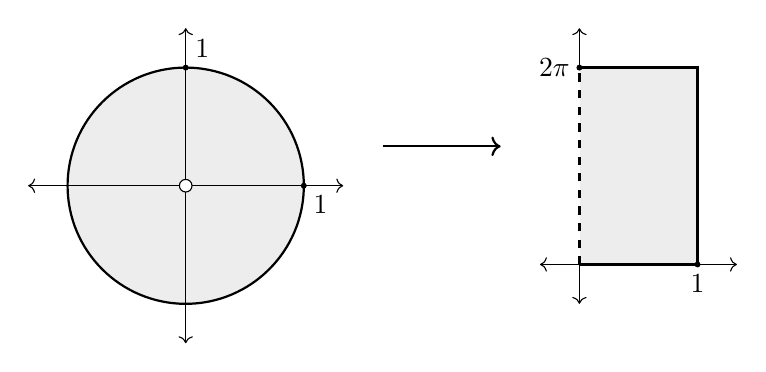
\begin{tikzpicture}
      \draw[thick, fill=lightgray] (0,0) circle (1.5); 
      \draw[<->] (-2,0)--(2,0);
      \draw[<->] (0,-2)--(0,2);
      \draw[fill=white] (0,0) circle (0.08);
      \draw[->, thick] (2.5,0.5)--(4, 0.5); 
      \draw[<->] (4.5,-1)--(7,-1);
      \draw[<->] (5,-1.5)--(5,2);
      \draw[white, fill=lightgray] (5,-1) rectangle (6.5,1.5);
      \draw[thick] (5,-1)--(6.5,-1)--(6.5,1.5)--(5,1.5);
      \draw[thick, dashed] (5,-1)--(5,1.5);
      \draw[fill] (6.5,-1) circle (0.03);
      \node[below] at (6.5,-1) {$1$};
      \node[left] at (5,1.5) {$2 \pi$};
      \draw[fill] (5, 1.5) circle (0.03);
      \draw[fill] (1.5,0) circle (0.03);
      \draw[fill] (0,1.5) circle (0.03);
      \node[below right] at (1.5,0) {$1$};
      \node[above right] at (0,1.5) {$1$};
  \end{tikzpicture}
  \end{center}

  If we are given an unbounded region $D \subset \mathbb{R}^2$, we can first create a bounded region and expand that region using a limit to cover all of $D$. 



\section{Surfaces}

\section{Integration of Forms}

\subsection{Line Integrals}

  \begin{definition}[Orientations, Simple Curves, Closed Curves]
  A path function $p: [a,b]\subset \mathbb{R} \longrightarrow \mathbb{R}^n$ determines a curve in $\mathbb{R}^n$ with endpoints $p(a)$ and $p(b)$. The direction the curve $p$ takes, that is from $p(a)$ to $p(b)$ in $\mathbb{R}^n$ is called the \textit{orientation} of $p$. A path or a curve with a defined orientation is called an \textit{oriented curve}. 

  A \textit{simple curve} $C$ to be the image of an injective piecewise $C^1$ map $c: I \subset \mathbb{R} \longrightarrow \mathbb{R}^3$. Since it is inejctive, it does not intersect itself, and $C$ is piecewise smooth in $\mathbb{R}^n$. If $I = [a,b]$, then $c(a)$ and $c(b)$ are the endpoints of the curve. A simple curve with an orientation is called an \textit{oriented simple curve}. 

  A closed curve $C$ is the image of piecewise $C^1$ map $c: [a,b] \longrightarrow \mathbb{R}^n$ such that $c(a) = c(b)$. That is, the endpoints of $C$ are equal. A \textit{simple closed curve} is a closed curve that is injective over the interval $[a,b)$. Note that a closed curve has two possible orientations. 
  \end{definition}

  If $C$ is an oriented simple curve or an oriented simple closed curve, then we can unambiguously define line integrals along them. 

  \begin{definition}
  Let $h$ be an injective function that takes $[\alpha,\beta] \subset \mathbb{R}$ to the interval $[a, b] \subset \mathbb{R}$. Given an oriented simple path function $p: [a,b]\subset \mathbb{R} \longrightarrow \mathbb{R}^n$, the composition
  \[\rho = p \circ h: [\alpha, \beta] \longrightarrow \mathbb{R}^n\]
  is called a \textit{reparamaterization} of $p$. Note that since $h$ is injective, it takes endpoints to endpoints. If $h$ preserves the direction in which the path travels, that is, if 
  \[(p \circ h)(\alpha) = a \text{ and } (p \circ h)(\beta) = b\]
  then $h$ is \textit{orientation preserving}. If
  \[(p \circ h)(\alpha) = b \text{ and } (p \circ h)(\beta) = a\]
  then $h$ is \textit{orientation reversing}. Note that a path $c$ having the same image as $p$ does not imply that $c$ is a reparamaterization of $p$, since $c$ may not be injective. 
  \begin{center}
      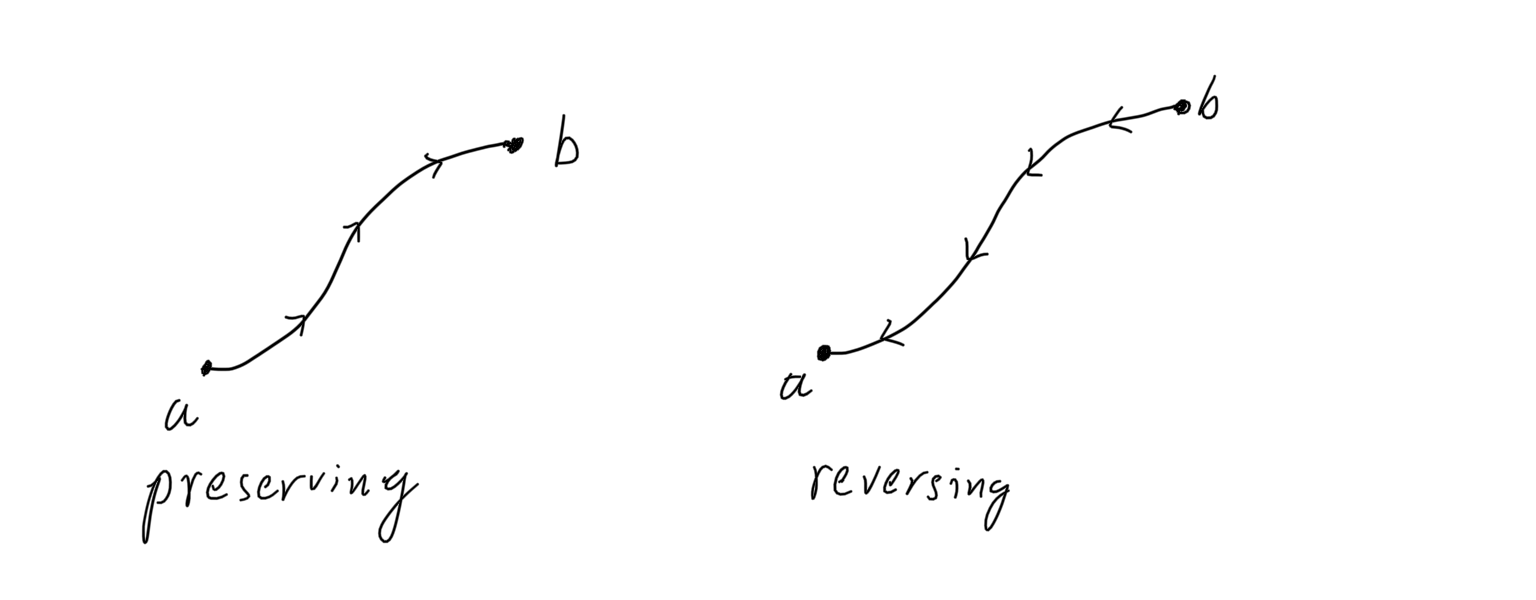
\includegraphics[scale=0.25]{img/Orientation_Preserving_Reversing.PNG}
  \end{center}
  \end{definition}

  \begin{definition}[Scalar Line Integral]
  Let $f: \mathbb{R}^n \longrightarrow \mathbb{R}$, which can be interpreted as a scalar field. Now define a $C^1$ path function 
  \[c: [a,b] \subset \mathbb{R} \longrightarrow \mathbb{R}^n \]
  such that the composition of functions
  \[f \circ c: [a, b] \subset \mathbb{R} \longrightarrow \mathbb{R}^n\]
  is continuous. Then, the \textit{path integral}, or \textit{scalar line integral}, of $f$ along the path $c$. is defined
  \begin{align*}
      \int_c f \;d s & = \int_a^b f\big(c(t)\big) ||c^\prime (t)|| \;d t \\
      & = \int_a^b f\big( x_1 (t), x_2 (t), ..., x_n (t)\big) ||c^\prime (t)|| \; d t
  \end{align*}
  If $c(t)$ is only piece-wise $C^1$, we can define the path integral by breaking $[a,b]$ into pieces over with $f\big( c(t)\big) ||c^\prime (t)||$ is continuous and then summing the integrals over the pieces. 
  That is, 
  \[\int_a^b f\big(c(t)\big) ||c^\prime (t)|| \;d t = \sum_{i = 0}^{n-1} \int_{\alpha_i}^{\alpha_{i+1}} f\big(c(t)\big) ||c^\prime (t)|| \; d t\]
  \end{definition}
  Note that since $f$ is a scalar-valued function, we can interpret a path integral as the sum of infinitesmal segments of the path $c$ having a weight determined by $f$ at each section. 
  If $f$ is a constant function outputting $1$ at every point, then the path integral just outputs the length of the path $c$ in $\mathbb{R}^n$. 
  \[L = \int_a^b f\big( c(t)\big) ||c^\prime (t)|| \; d t = \int_a^b ||c^\prime (t)|| \; d t\]

  \begin{definition}[Vector Line Integral]
  Let $F: \mathbb{R}^n \longrightarrow \mathbb{R}^n$ be a vector field on $\mathbb{R}^n$ that is continuous on the $C^1$ oriented path $c: [a, b] \subset \mathbb{R} \longrightarrow \mathbb{R}^n$. The \textit{line integral} of $F$ along $c$ is defined by the formula 
  \[\int_c F \cdot d s = \int_a^b F\big( c(t)\big) \cdot c^\prime (t) \; d t\]
  where $\cdot$ represents the dot product of $F$ with $c^\prime$ over the interval $[a,b]$. It is also commonly written in differential notation, 
  \[\int_c F \cdot ds = \int_c F \cdot (dx_1, \ldots, d x_n) = \int_c F_1 dx_1 + F_2 dx_2 + \ldots F_n dx_n\]
  \begin{center}
      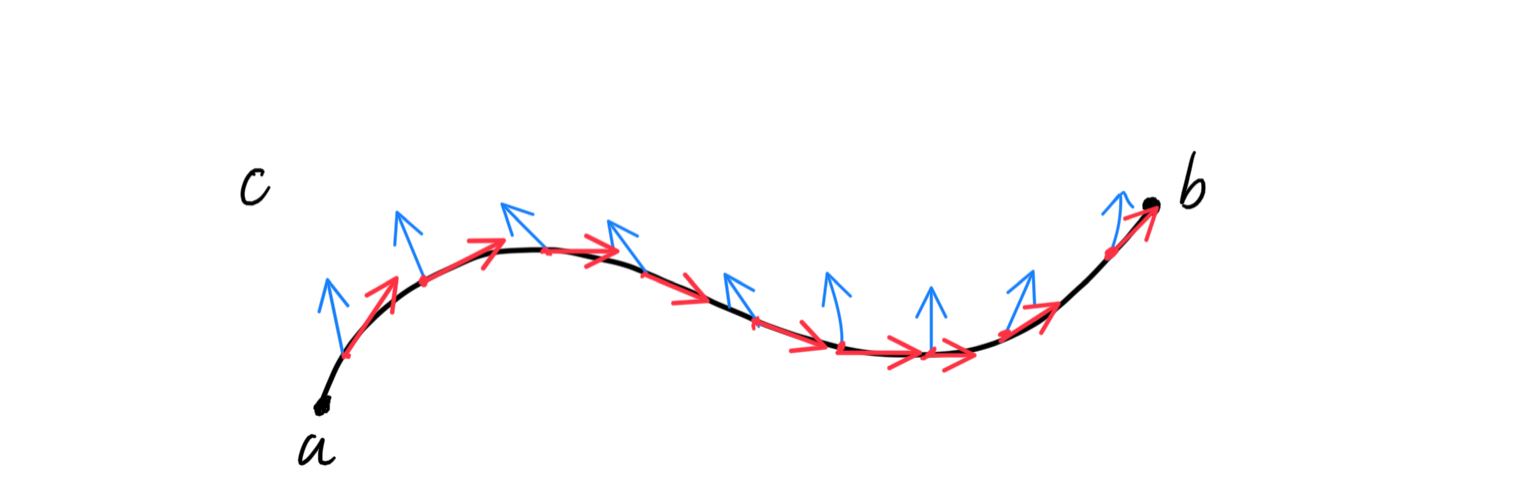
\includegraphics[scale=0.27]{img/Vector_Line_Integral.PNG}
  \end{center}
   Similarly with path integrals, we can also define line integrals as the sum of integrals over piece-wise continuous sections of $c$. That is, given an oriented curve $C$ made up of several oriented component curves $C_i$, $i = 1, 2, ..., k$, we can paramaterize $C$ by paramaterizing the pieces $C_i$'s separately. Thus, we can treat $C = C_1 + ... C_k$ and get
  \[\int_C F \cdot d s = \sum_{i = 1}^k \int_{C_i} F \cdot d s\]
  Note that a vector line integral is a generalization of scalar line integrals, so any results holding for vector line integrals also holds for their scalar counterpart. 
  \end{definition}

  \begin{example}[Work]
  In mechanics, work $W$ is defined as 
  \[W = F \cdot d\]
  where $F$ is force and $d$ is displacement. With this knowledge, the reader can easily see that the work done by vector field $F$ on a particle traveling along a path $c$ from time $a$ to time $b$ can be calculated by the line integral
  \begin{align*}
      W & = \int_a^b F\big( c(t)\big) \cdot c^\prime (t) \; d t \\
      & = \int_c F_1 dx + F_2 dy + F_3 dz
  \end{align*}
  \end{example}

  \begin{theorem}[Invariance of Path Paramaterizations on Vector Line Integrals]
  Let $F$ be a vector field and $f$ be a scalar field, both continuous on the $C^1$ path function $p: [a,b] \longrightarrow \mathbb{R}^n$ and let $q: [\alpha, \beta] \longrightarrow \mathbb{R}^n$ be a reparamaterization of $p$. Then, 
  \begin{align*}
      q \text{ is orientation preserving} & \implies \int_p F \cdot d s = \int_q F \cdot d s \\
      q \text{ is orientation reversing} & \implies \int_p F \cdot d s = - \int_q F \cdot d s
  \end{align*}
  \end{theorem}

\subsection{Conservative Vector Fields}

  We now introduce a fundamental theorem about line integrals over gradient fields. Recall the fundamental theorem of calculus and it's equivalent form. 

  \begin{theorem}[Fundamental Theorem of Single Variable Calculus]
  Let function $\nabla g: \mathbb{R} \longrightarrow \mathbb{R}$ be the gradient of the single variable $C^1$ function $g: \mathbb{R} \longrightarrow \mathbb{R}$; that is, $\nabla g$ is a conservative vector field on $\mathbb{R}$. Then, 
  \[\int_a^b \nabla g (x) \,dx = g(b) - g(a)\]
  Note that in the single variable case, 
  \[\frac{d}{dx} g(x) = \nabla g(x)\]
  This means that the value of the integral of $\nabla g$ only depends on the value of $g$ at the endpoints of the interval $[a,b]$. 
  \end{theorem}

  We can extend this to line integrals for functions mapping $\mathbb{R}^n$ to $\mathbb{R}$. 

  \begin{theorem}[Invariance of Line Integrals in Conservative Vector Fields]
  Given that $F: \mathbb{R}^n \longrightarrow \mathbb{R}^n$ is a $C^1$ conservative vector field with $\nabla f = F$ for $C^2$ function $f: \mathbb{R}^n \longrightarrow \mathbb{R}$ and path function $p: [a,b] \longrightarrow \mathbb{R}^n$ is a piecewise $C^1$ path, then 
  \[\int_p F \cdot d s = \int_p \nabla f \cdot d s = f\big(p(b)\big) - f\big(p(a)\big)\]
  That is, the line integral of any path in a conservative vector field is dependent on the value of $f$ at the endpoints $p(a)$ and $p(b)$. 
  \begin{center}
      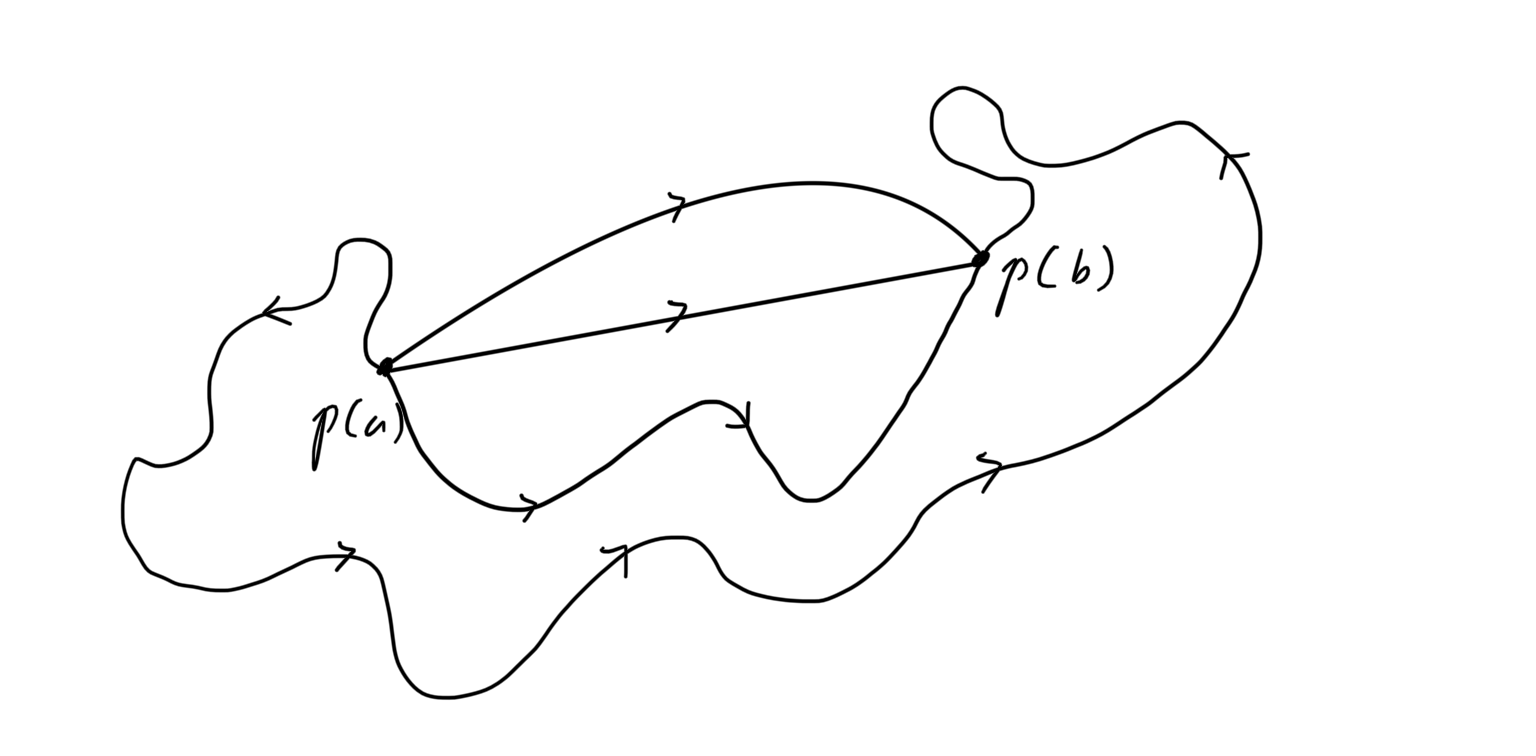
\includegraphics[scale=0.2]{img/Line_Integral_Independence_of_path.PNG}
  \end{center}
  \end{theorem}

  In physics, calculating the work done by a force represented by a vector field requires us to know the path that it travels through. 
  \[W = \int_p F \cdot ds\]
  However, in many cases $F$ is assumed to be conservative, so it is only necessary that we find the displacement of the particle from its endpoints, resulting in the simplification of the formula.  
  \[W = \int_p \nabla f \cdot ds = f\big( p(b)\big) - f \big(p(a)\big)\]

  \begin{corollary}[Equivalent Conditions for Vector Field to be Conservative]
  The following conditions are equivalent: 
  \begin{enumerate}
      \item $F: \mathbb{R}^n \longrightarrow \mathbb{R}^n$ is a conservative vector field. 
      \item The line integral of $F: \mathbb{R}^n \longrightarrow \mathbb{R}^n$ in curve $C$ is path independent; that is, if $C_1$ and $C_2$ are two paramaterizations of $C$, 
      \[\int_{C_1} F \cdot ds = \int_{C_2} F \cdot ds\]
      \item Given that $C$ is a closed loop, the line integral of $F: \mathbb{R}^n \longrightarrow \mathbb{R}^n$ across $C$ is $0$. 
      \[\oint_C F \cdot ds = 0\]
      \item The curl of $F: \mathbb{R}^3 \longrightarrow \mathbb{R}^3$ vanishes
      \[\curl{F} = \nabla \times F = \begin{pmatrix}
      \frac{\partial F}{\partial x} \\\frac{\partial F}{\partial y} \\\frac{\partial F}{\partial z} 
      \end{pmatrix} \times \begin{pmatrix}
      F_1\\F_2\\F_3
      \end{pmatrix}= 0\]
      \item The following partial derivatives of $F: \mathbb{R}^2 \longrightarrow \mathbb{R}^2$ are equal
      \[\frac{\partial F_1}{\partial y} = \frac{\partial F_2}{\partial x}\]
  \end{enumerate}
  \end{corollary}

  We can develop a bit of intuition to determine whether a vector field is conservative or not. If vector field $F$ is conservative, then there exists a smooth scalar field $f$ such that $\nabla f = F$. For each latitude and longitude on a certain map, we can give it an altitude as a function of those coordinates (picture a map with a bunch of hills and valleys). The gradient and thus the vector field is all the vectors that point in the direction of highest ascent. he vector field is all the vectors that point in the direction of highest ascent. Extending the metaphor the path integral is like starting on at a point and climbing the hills and valleys, creating work as you go up a hill (proportional to the steepness and thus the dot product of your motion vector with the gradient vector field in the path integral) and decreasing the work you put in by going down a hill. Since the path is closed, it is like you are going up and down the same amount overall, so the path integral is zero. Following this analogy, the vector field determined by this function (marked as arrows in the $x, y$ plane) is conservative. 
  \begin{center}
      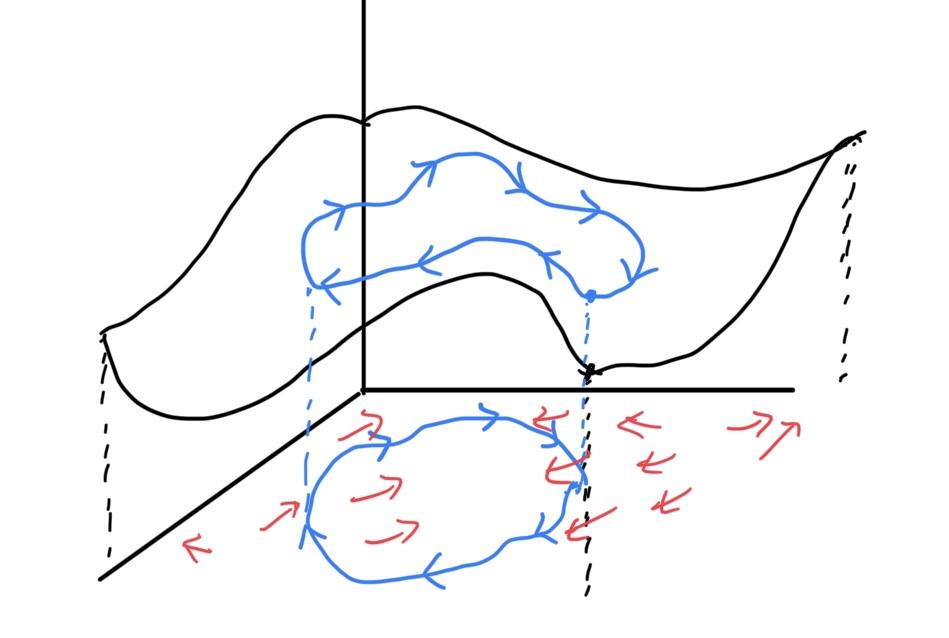
\includegraphics[scale=0.28]{img/Conservative_Vector_Field.jpg}
  \end{center}
  If we can construct a closed loop around $F$ where the line integral is nonzero, then it means that we have ended up at a "higher" or "lower" (altitude) at the same point. This means that rather than being a certain landscape, there exist different "levels" of values at one point, like a spiraling staircase. For example, look at the solenoidal vector field below, where we can construct a closed loop (a circle going around the origin counterclockwise). There is no "surface" that can be defined such that it contains the solenoid. 
  \begin{center}
      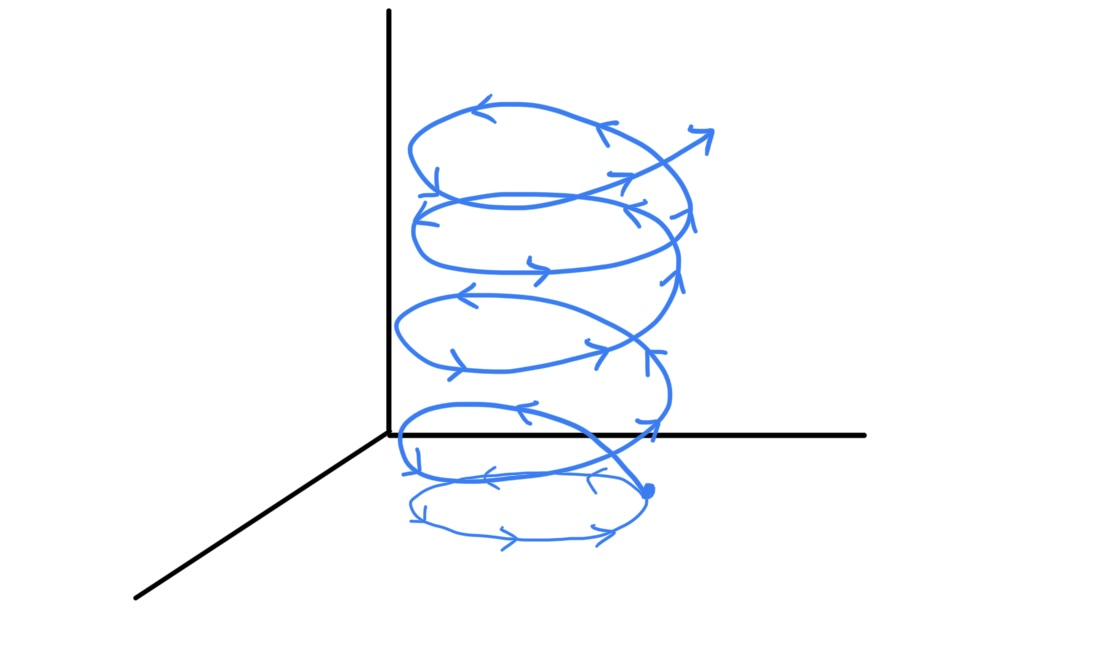
\includegraphics[scale=0.28]{img/Solenoid_nonconservative.jpg}
  \end{center}
  Clearly, as a particle travels through the vector field along the path, it does positive work while it has zero displacement, and clearly, there exists no function that can output both these values as determined by vector field $F$. 

  \begin{theorem}[Helmholtz Decomposition]
  Let $F: \mathbb{R}^3 \longrightarrow \mathbb{R}^3$ be a $C^2$ vector field. Then, $F$ can be decomposed into a curl-free component and a divergence-free component. That is, there exists vector fields $A$ and $\Phi$
  \[F = - \nabla \cdot \Phi + \nabla \times A\]
  \end{theorem}

  \subsubsection{Curvature}
  \begin{definition}[Curvature at a Point]
  Let $c: [a, b] \longrightarrow C \subset \mathbb{R}^3$ be a unit-speed paramaterization of $C$, meaning that $||c^\prime (t)|| = 1$ for all $t \in [a,b]$, and let $p = c(t_0)$ be a point in $C$. The \textit{curvature} $\kappa(p)$ at $p$ is a mapping defined
  \[\kappa: C \longrightarrow \mathbb{R}, \;\; \kappa(p) \equiv ||c^{\prime \prime} (t_0)||\]
  Notice that since we require a unit speed paramaterization of $C$, we do not need to worry about how a given curve is paramaterized. 
  \end{definition}

  Since the curvature is defined pointwise for each point in curve $C$, we can integrate over all the curvatures in $C$ to define the total curvature. 

  \begin{definition}[Total Curvature]
  The \textit{total curvature} of a curve $c: [a,b] \longrightarrow C \subset \mathbb{R}^3$ is the scalar line integral 
  \[\int_C \kappa \, ds\]
  \end{definition}

  We now present an important theorem in differential geometry. 
  \begin{theorem}[Fary-Milnor Theorem]
  Given a unit speed paramaterization $c: [a,b] \longrightarrow C \subset \mathbb{R}^3$, if $C$ is closed (that is, $c(a)=c(b)$), then 
  \[\oint_C \kappa\, ds \geq 2 \pi\]
  and equals $2\pi$ only when $C$ is a circle. Furthermore, if $C$ is a closed space curve with 
  \[\oint_C \kappa\, ds \leq 4\pi\]
  then $C$ is "unknotted." That is, $C$ can be continuously deformed without every intersecting itself into a planar circle. Therefore, for knotted curves $C$, we have
  \[\oint_C \kappa \, ds > 4\pi\]
  \end{theorem}

\subsection{Surface Integrals}

  Surface integrals are the $2$-dimensional analogue, or the double integral version, of line integrals. It is the integration of surfaces. 

  \subsubsection{2-Dimensional Paramaterizations of Surfaces}
  Just like how we create path functions using a paramaterization function $p: [a, b] \subset \mathbb{R} \longrightarrow \mathbb{R}^n$, we can parameterize surfaces by defining a function 
  \[\varphi: D \subset \mathbb{R}^2 \longrightarrow \mathbb{R}^n, \;\;\; \varphi (u, v) \equiv \begin{pmatrix} x_1 (u, v) \\ \vdots \\ x_n (u, v) \end{pmatrix}\]
  The surface 
  \[S = \varphi(D)\]
  corresponding to the function $\varphi$ is its image. If $\varphi$ is differentiable or is of class $C^1$, then we call $S$ a \textit{differentiable} or $C^1$ surface, respectively. 

  For those that are familiar with differential geometry, this makes every paramaterized surface a 2-manifold induced by the single homeormophism $\varphi$. In fact, it is more than just locally homeomorphic; it is \textit{globally} homeomorphic. 


  \begin{definition}[Tangent Vectors of Surfaces Embedded in $\mathbb{R}^3$]
  Given surface paramaterization 
  \[\varphi: \mathbb{R}^2 \longrightarrow \mathbb{R}^3, \;\;\; \varphi(u, v) \equiv \begin{pmatrix}
  x (u, v) \\ y(u, v) \\ z(u, v) 
  \end{pmatrix}\]
  it is visually clear that there can be up to two linearly independent tangent vectors at a point on the surface $S$. We can calculate these two vectors by embedding two nonparallel paths in $D \subset \mathbb{R}^2$ and taking the derivative with respect to a point traveling through these paths, which would give us a tangent vector on $S$. To keep things simple, we take the partial derivatives with respect to $u$ and $v$. 
  \begin{center}
      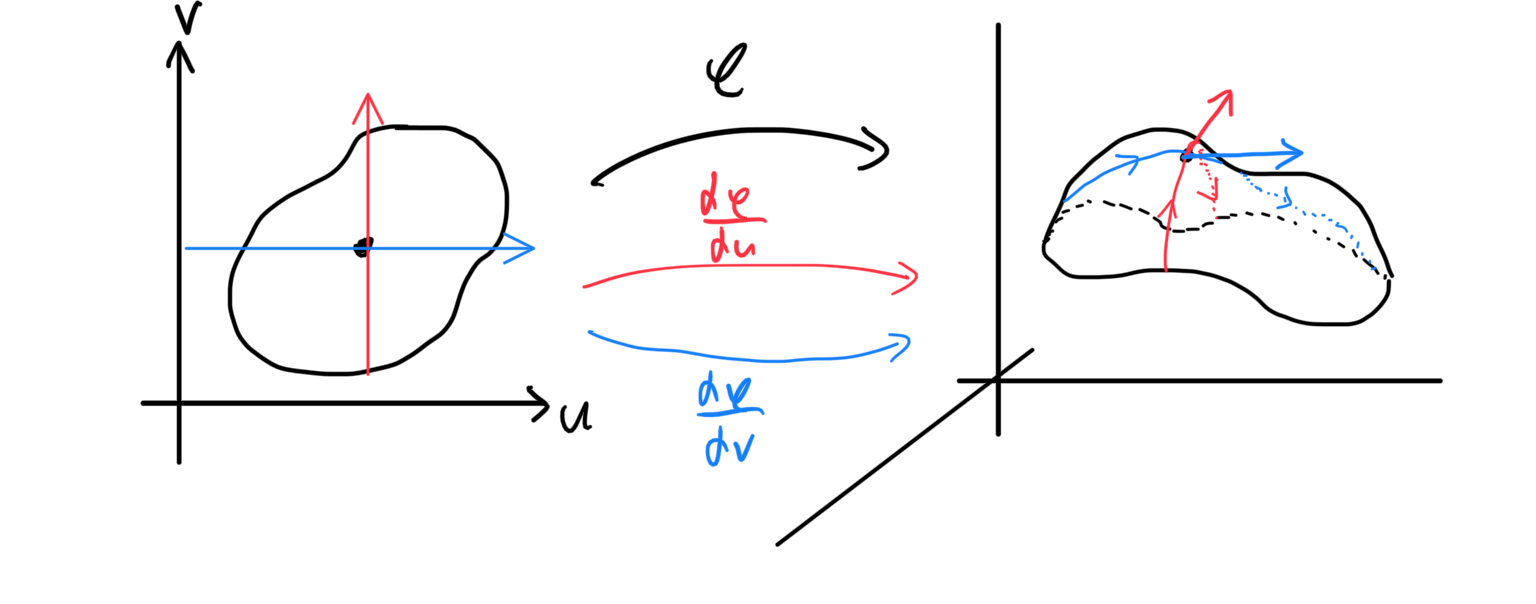
\includegraphics[scale=0.28]{img/Partial_Derivatives_with_respect_to_U_V.PNG}
  \end{center}
  Clearly, these paths are functions 
  \begin{align*}
      \frac{\partial \varphi}{\partial u} \equiv \begin{pmatrix}
       \frac{\partial x}{\partial u} \\ \frac{\partial y}{\partial u} \\ \frac{\partial z}{\partial u}
      \end{pmatrix} : \mathbb{R}^2 \longrightarrow \mathbb{R}^3\\
      \frac{\partial \varphi}{\partial v} \equiv \begin{pmatrix}
       \frac{\partial x}{\partial v} \\ \frac{\partial y}{\partial v} \\ \frac{\partial z}{\partial v}
      \end{pmatrix} : \mathbb{R}^2 \longrightarrow \mathbb{R}^3
  \end{align*}
  where 
  \[\frac{\partial \varphi}{\partial u} (u_0 ,v_0), \; \frac{\partial \varphi}{\partial v} (u_0, v_0)\]
  represent two vectors in $\mathbb{R}^3$ that are tangent to $S$ at the point $\varphi(u_0, v_0) \in \mathbb{R}^3$. 
  \end{definition}

  We must make sure that the surface $S$ is smooth in the sense that (informally) there aren't any wrinkles, points, folds, or self-intersections in such a way that the tangent plane to the surface is not well-defined. 

  \begin{definition}[Regular Surfaces]
  To formalize this concept, we say that $S$ is \textit{regular}, or \textit{smooth}, at point $(u_0, v_0)$ if
  \[\frac{\partial \varphi}{\partial u} \times \frac{\partial \varphi}{\partial v} \neq 0\]
  where $\times$ is the Euclidean cross product. That is, if the vector that is orthogonal to the two tangent vectors is well defined at a point, the surface is said to be smooth at that point. Note that $\frac{\partial \varphi}{\partial u}$ is parallel to $\frac{\partial \varphi}{\partial v}$ if and only if their cross product is $0$. 
  \begin{center}
      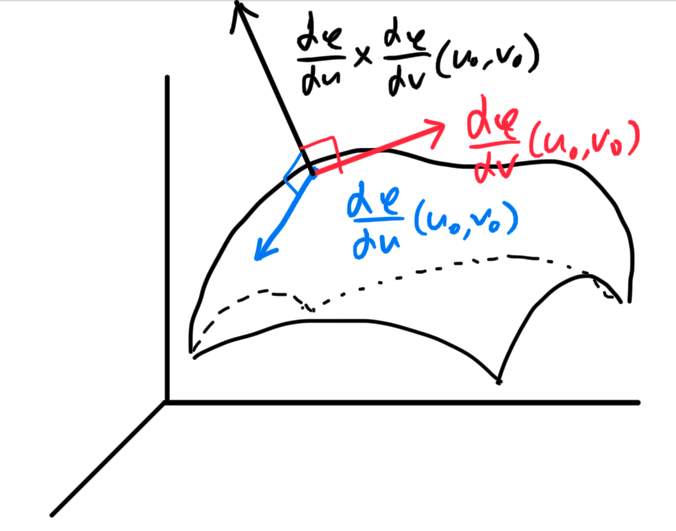
\includegraphics[scale=0.3]{img/Cross_Product_Regular_Surfaces.PNG}
  \end{center}
  It is quite clear that $(\frac{\partial \varphi}{\partial u} \times \frac{\partial \varphi}{\partial v})(u_0, v_0) \neq 0 \implies \frac{\partial \varphi}{\partial u}$ and $\frac{\partial \varphi}{\partial v}$ are linearly independent. This means that an entire span of tangent vectors, i.e. a tangent plane, of the surface $S$ at $\varphi(u_0, v_0)$ exists. 
  $S$ is said to be \textit{regular} if it is regular at all points $\varphi(u_0, v_0) \in S$. 
  \end{definition}

  In fact, the tangent plane at $\varphi(u_0, v_0)$ is the set of points 
  \[\{\varphi(u_0, v_0) + \frac{\partial \varphi}{\partial u} (u_0, v_0) c_1 + \frac{\partial \varphi}{\partial v} (u_0, v_0) c_2 \; | \; c_1, c_2 \in \mathbb{R} \}\]
  which is precisely the affine tangent plane spanned by $T_u$ and $T_v$. Note also that the vector $T_u \times T_v$, if nonzero, is normal to this plane, which leads to this equivalent definition. 

  \begin{definition}[Tangent Planes of Surfaces]
  Given a paramaterized surface $\varphi: D \subset \mathbb{R}^2 \longrightarrow \mathbb{R}^3$ that is regular at $\varphi(u_0, v_0)$, the tangent plane of the surface $S$ at $\varphi(u_0, v_0) = (x_0, y_0, z_0)$ is defined
  \[\{(x, y, z) \in \mathbb{R}^3 \;|\; (x-x_0, y-y_0, z-z_0) \cdot n = 0\}\]
  where $n = (\frac{\partial \varphi}{\partial u} \times \frac{\partial \varphi}{\partial v})(u_0, v_0)$. 
  \end{definition}

  We finally construct the concept of signed areas before defining surface integration. 
  We have all the tools we need to calculate surface areas, but remember that integration also covers the concept of \textit{signed areas}, which could be negative. In order to define this, we define the concept of orientation on surfaces. 

  \subsubsection{Orientation of Surfaces}

  \begin{definition}[Oriented Surfaces]
  An \textit{oriented surface} is a two-sided surface with one side specified as the \textit{outside/positive} side and the other side as the \textit{inside/negative} side. Note that an oriented surface is not guaranteed to have two sides (e.g. a Mobius strip). To ensure that there exist two sides, $S$ must be regular. 

  Surprisingly, a paramaterization does not have an intrinsic orientation. Rather, we determine the orientation ourselves by choosing a unit vector that generally points towards the outside of the surface $S$. Again, this choice is arbitrary, but it is customary to choose a vector that generally points "out." Either way, the orientation (unit) vector at every point $\varphi(u, v) \in S$, denoted as $n$, is 
  \[n\big(\varphi(u, v)\big) = \pm \frac{\frac{\partial \varphi}{\partial u} \times \frac{\partial \varphi}{\partial v}}{\big|\big|\frac{\partial \varphi}{\partial u} \times \frac{\partial \varphi}{\partial v}\big|\big|}\]
  which can be visually calculated using the right hand rule. 
  \begin{center}
      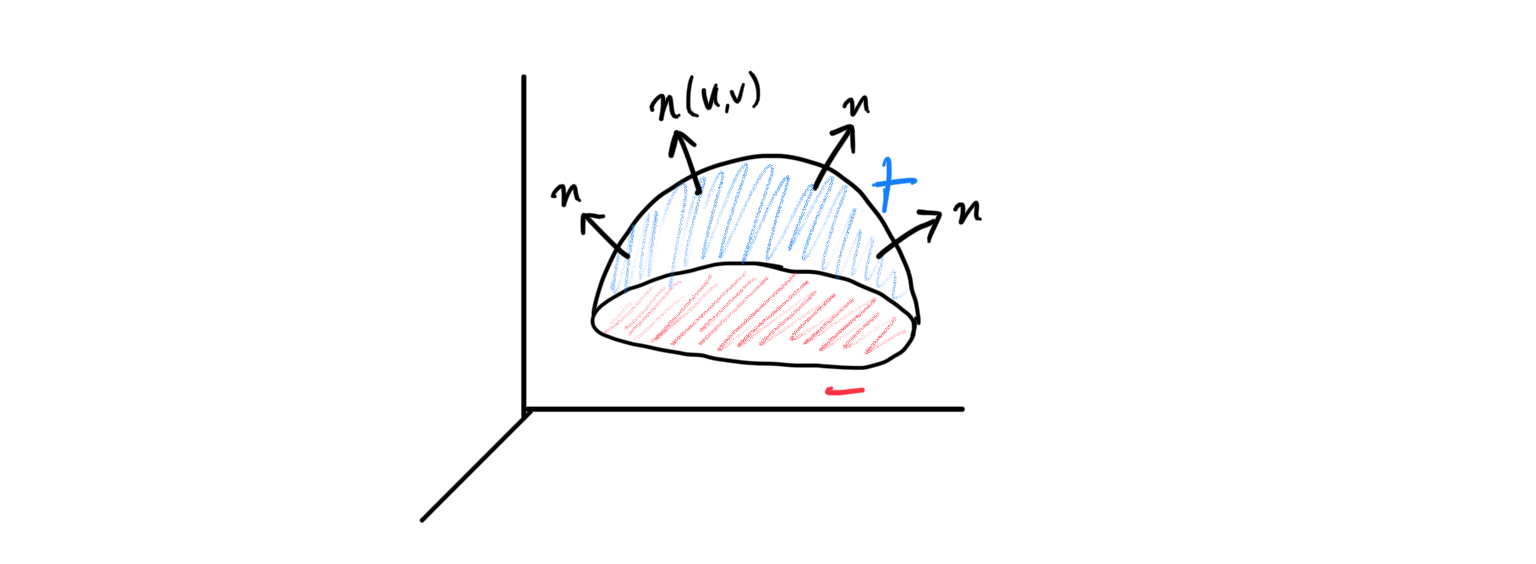
\includegraphics[scale=0.23]{img/Orientation_Unit_Vector.PNG}
  \end{center}
  \end{definition}

  \begin{definition}[Orientation Preserving, Reversing Paramaterizations]
  Given an oriented surface $S$ with its positive side determined by the direction of unit vector $n\big( \varphi(u,v)\big)$, the paramaterization $\varphi$ is said to be \textit{orientation preserving} if 
  \[n \big( \varphi(u, v)\big) = \frac{\frac{\partial \varphi}{\partial u} \times \frac{\partial \varphi}{\partial v}}{\big|\big|\frac{\partial \varphi}{\partial u} \times \frac{\partial \varphi}{\partial v}\big|\big|}\]
  and \textit{orientation reversing} if
  \[n \big( \varphi(u, v)\big) = - \frac{\frac{\partial \varphi}{\partial u} \times \frac{\partial \varphi}{\partial v}}{\big|\big|\frac{\partial \varphi}{\partial u} \times \frac{\partial \varphi}{\partial v}\big|\big|}\]
  \end{definition}

  So, to find whether a paramaterization is orientation preserving or reversing, it suffices to find the cross product $T_u \times T_v$ and see if it points in the same direction of the normal vector $n$ (which should have already been determined when deciding the orientation of $S$). 

  Given a paramaterization $\varphi$ and an un-oriented surface $S$, we can also just construct $\varphi$ to be orientation-preserving (or reversing) by \textit{defining} the normal vector $n$ to be 
  \[n\big( \varphi(u, v)\big) = \frac{\frac{\partial \varphi}{\partial u} \times \frac{\partial \varphi}{\partial v}}{\big|\big|\frac{\partial \varphi}{\partial u} \times \frac{\partial \varphi}{\partial v}\big|\big|} \;\; \bigg( \text{or } n\big( \varphi(u, v)\big) = - \frac{\frac{\partial \varphi}{\partial u} \times \frac{\partial \varphi}{\partial v}}{\big|\big|\frac{\partial \varphi}{\partial u} \times \frac{\partial \varphi}{\partial v}\big|\big|} \bigg)\]
  So rather than finding out whether a paramaterization $\varphi$ is orientation preserving or reversing by comparing $T_u \times T_v$ with $n$, we have defined $n$ in a way such that $\varphi$ must be orientation preserving (or reversing). We can utilize these tools of paramaterization to now define the surface integral. 

  \subsubsection{Scalar, Vector Surface Integrals}

  A physical interpretation of a scalar surface integral is the weighted surface area of a certain surface. 

  \begin{definition}[Scalar Surface Integrals]
  Let $f: \mathbb{R}^3 \longrightarrow \mathbb{R}$ be a $C^1$ scalar field defined on a paramaterized surface $S \subset \mathbb{R}^3$ with paramaterization $\varphi: D \subset \mathbb{R}^2 \longrightarrow \mathbb{R}^3$. That is, $\varphi(D) = S$. We define the integral $f$ over $S$ to be
  \begin{align*}
      \iint_S f \; dS & = \iint_S f(x, y, z) \; dS \\
      & = \iint_D f\big( \varphi(u, v)\big) \bigg|\bigg|\frac{\partial \varphi}{\partial u} \times \frac{\partial \varphi}{\partial v}\bigg|\bigg| \; du \,dv
  \end{align*}
  Note that this will require us to transform $f$, a function of $x, y, z$, into the function $f \circ \varphi$ of $u, v$. Additionally, if the paramaterization of the surface $S$ is not defined, then it one must be constructed. It is also clear that if $S$ is a union of surfaces $S_i$, then its surface integral is the sum of the surface integrals of the $S_i$'s. 
  \end{definition}

  Letting the scalar field $f$ be the constant field equal to $1$, the scalar surface integral measures the surface area of $S$. 
  \[A(S) = \iint_S \; dS = \iint_D \Big|\Big|\frac{\partial \varphi}{\partial u} \times \frac{\partial \varphi}{\partial v}\Big|\Big| \; du\, dv\]
  It is easy to see that the orientation of the paramaterization $\varphi$ does not affect scalar surface integrals, since the sign of the orientation gets nullified by the absolute value sign over $||\frac{\partial \varphi}{\partial u} \times \frac{\partial \varphi}{\partial v}||$. 

  Its physical interpretation is to measure the rate at which a fluid (determined by a vector field $F$) is crossing a given surface $S$. It also has many applications in electromagnetism. 

  \begin{definition}[Vector Surface Integrals]
  Let $F$ be a vector field defined on surface $S$, the image of a paramaterized surface $\varphi$. The \textit{surface integral} of $F$ over $S$ is defined below, which is equivalent to summing up the dot product of the vector field and the normal vector to the surface. 
  \begin{center}
      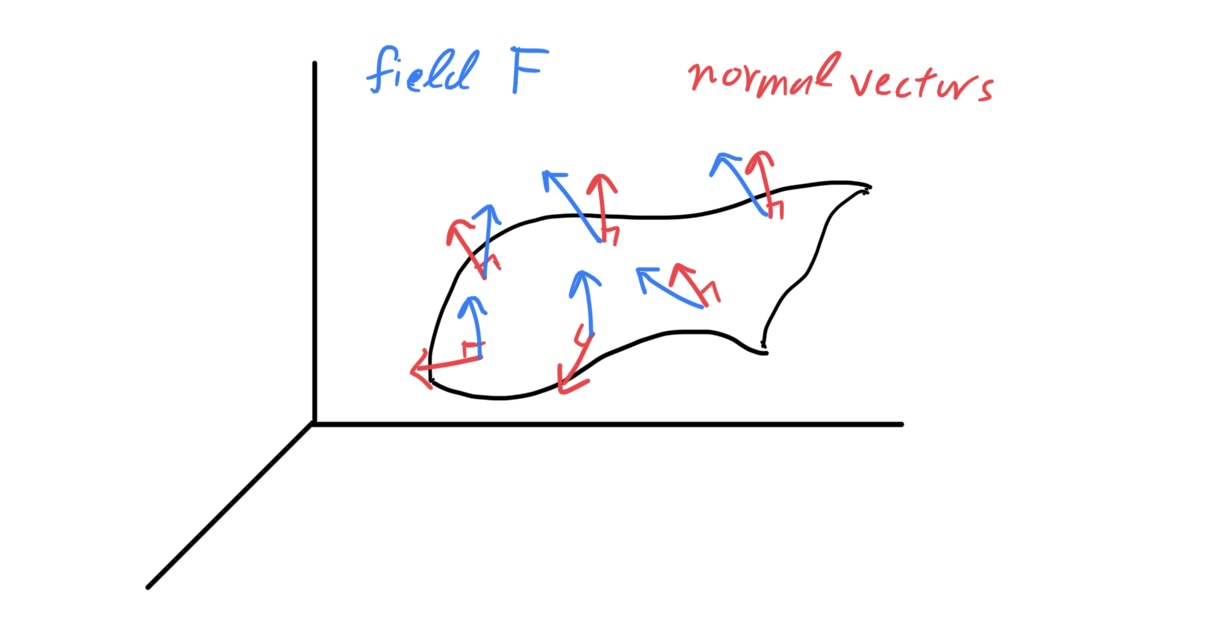
\includegraphics[scale=0.3]{img/Vector_Surface_Integral.jpg}
  \end{center}
  It can be calculated with the following formulas by converting it into a scalar surface integral where the scalar field is the value of the dot product of the vector field with the normal vectors of the surface. 
  \begin{align*}
      \iint_{S} F \cdot d S & = \iint_S (F \cdot n) \; dS \\
      & = \iint_D \Bigg( F\big( \varphi(u, v)\big) \cdot \frac{\frac{\partial \varphi}{\partial u} \times \frac{\partial \varphi}{\partial v}}{\Big|\Big|\frac{\partial \varphi}{\partial u} \times \frac{\partial \varphi}{\partial v} \Big|\Big|} \Bigg) \, \bigg|\bigg|\frac{\partial \varphi}{\partial u} \times \frac{\partial \varphi}{\partial v}\bigg|\bigg|\; du\,dv \\
      & = \iint_D F\big(\varphi(u, v)\big) \cdot \bigg( \frac{\partial \varphi}{\partial u} \times \frac{\partial \varphi}{\partial v}\bigg) \; du\,dv
  \end{align*}
  \end{definition}

  Since we are now talking about vector fields, the orientation of the paramaterization is now significant. Visually, if the orientation of the surface $S$ generally aligns with the vector field $F$, then the integral will be positive (since two vectors $\alpha, \beta$ generally pointing in the same direction implies that $\alpha \cdot \beta > 0$). The orientation of the paramaterization, which is dependent on $\frac{\partial \varphi}{\partial u} \times \frac{\partial \varphi}{\partial v}$, determines the direction of the normal vector $n$ (since it is defined to be $(\frac{\partial \varphi}{\partial u} \times \frac{\partial \varphi}{\partial v}) / \big|\big|\frac{\partial \varphi}{\partial u} \times \frac{\partial \varphi}{\partial v}\big|\big|$. Therefore, changing the orientation of $\varphi$ will reverse the direction of $n$, which will then reverse the sign of the integral since $n$ now points in the opposite direction of the vector field $F$ than it previously did (by reversing the sign of the dot products). This is formalized in the theorem below. 

  \begin{theorem}[Invariance of Surface Paramaterizations on Vector Surface Integrals]
  Let $S$ be an oriented surface and let $\varphi_1$ and $\varphi_2$ be two regular paramaterizations with $F$ a continuous vector field defined on $S$. Then, assuming $\varphi_1$ is orientation preserving, 
  \begin{align*}
      \varphi_2 \text{ is orientation preserving } & \implies \iint_{\varphi_1} F \cdot d S = \iint_{\varphi_2} F \cdot d S \\
      \varphi_2 \text{ is orientation reversing } & \implies - \iint_{\varphi_1} F \cdot d S = \iint_{\varphi_2} F \cdot d S 
  \end{align*}
  \end{theorem}

  \subsubsection{Surface Integrals over Graphs}
  Given that we have the graph of a function $g: \mathbb{R}^2 \longrightarrow \mathbb{R}$ rather than a general surface, we can paramaterize it simply as
  \[\varphi(u, v) \equiv \big(u, v, g(u, v) \big)\]
  \begin{center}
      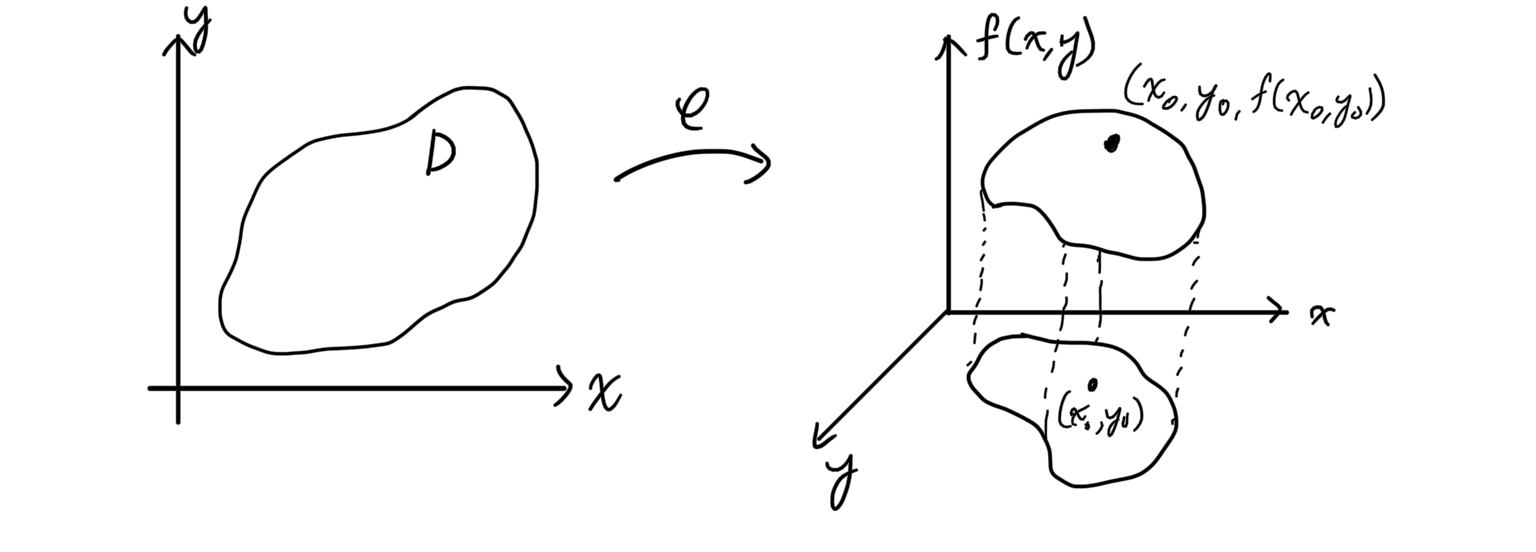
\includegraphics[scale=0.25]{img/Paramaterize_Surfaces_as_Graphs.PNG}
  \end{center}
  This means that 
  \[\frac{\partial \varphi}{\partial u} \times \frac{\partial \varphi}{\partial v} = 
  \begin{pmatrix}
  -\frac{\partial g}{\partial u} \\ -\frac{\partial g}{\partial v} \\ 1
  \end{pmatrix} \implies \bigg|\bigg|\frac{\partial \varphi}{\partial u} \times \frac{\partial \varphi}{\partial v} \bigg|\bigg| = \sqrt{1 + \Big(\frac{\partial g}{\partial u}\Big)^2 + \Big( \frac{\partial g}{\partial v}\Big)^2}\]
  So we can simplify the equation for the surface area $S$ of the graph of $g$ over the region $D$ in the $x y$-plane, as 
  \begin{align*}
      A(S) & = \iint_S \; d S = \iint_D \bigg|\bigg|\frac{\partial \varphi}{\partial u} \times \frac{\partial \varphi}{\partial v} \bigg|\bigg| \; d A \\
      & = \iint_D \sqrt{1 + \Big(\frac{\partial g}{\partial u}\Big)^2 + \Big( \frac{\partial g}{\partial v}\Big)^2} \; d u \, d v
  \end{align*}
  With the same $g$, we can find the weighed surface area of $S$ over the scalar function $f: \mathbb{R}^3 \longrightarrow \mathbb{R}$ with the formula
  \[\iint_S f \; d S = \iint_D f\big(u, v, g(u, v)\big) \sqrt{1 + \Big(\frac{\partial g}{\partial u}\Big)^2 + \Big( \frac{\partial g}{\partial v}\Big)^2} \; d u \, d v\]
  Finally, with the same graph $g$, the surface integral over the vector field $F$ is
  \begin{align*}
      \iint_S F \cdot d S & = \iint_D F\big(\varphi(u, v)\big) \cdot \bigg( \frac{\partial \varphi}{\partial u} \times \frac{\partial \varphi}{\partial v}\bigg) \; d u \, d v \\
      & = \iint_D \bigg( F_1(u, v) \Big(- \frac{\partial g}{\partial u}\Big) + F_2 (u, v) \Big( - \frac{\partial g}{\partial v} \Big) + F_3 (u, v) \bigg) \; d u \, d v
  \end{align*}

\subsection{Integral Theorems}

  Recall the differential notation for writing line integrals. For 2 and 3 dimensions, it is written as
  \begin{align*}
      & \int_C F \cdot d s = \int_C F \cdot (d x, d y) = \int_C F_1 \, d x + F_2 \, d y \\
      & \int_C F \cdot d s = \int_C F \cdot (d x, d y, d z) = \int_C F_1 \, d x + F_2 \, d y + F_3 \, d z 
  \end{align*}
  \subsubsection{Green's Theorem}
  Green's Theorem gives the relationship between a line integral around a simple closed curve $C$ and a double integral over the plane region $D$ bounded by $C$. 

  \begin{theorem}[Green's Theorem in $\mathbb{R}^2$]
  Let there be a 2-dimensional $C^1$ vector field $F$ on $\mathbb{R}^2$ defined on a simple oriented closed piecewise-smooth curve $C$ and its bounded region $D \subset \mathbb{R}^2$ (that is, $C = \partial D$). Let the orientation of the path of $C$ be such that it is traveling \textit{counterclockwise}, i.e. a point traveling through $C$ would see the region $D$ to its \textit{left}, denoted as $C^+$ and the clockwise orientation as $C^-$.  Then, 
  \[\oint_{C^+} F_1 \, d x + F_2 \, d y = \iint_D \bigg( \frac{\partial F_2}{\partial x} - \frac{\partial F_1}{\partial y} \bigg) \; d x \, d y\]
  By reversing the orientation, it is clear that we have
  \[\oint_{C^-} F_1 \, d x + F_2 \, d y = - \iint_D \bigg( \frac{\partial F_2}{\partial x} - \frac{\partial F_1}{\partial y} \bigg) \; d x \, d y\]
  Note that this theorem is expressed in terms of the components of the vector field $F$. 
  \begin{center}
  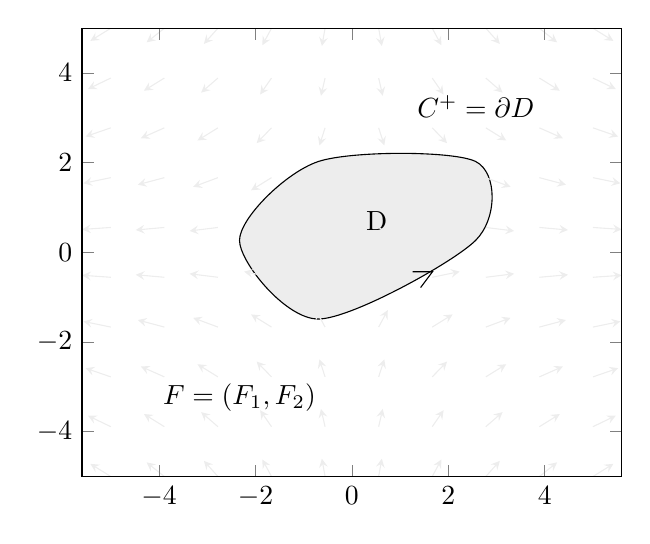
\begin{tikzpicture}
      \draw[fill=lightgray] plot [smooth cycle] coordinates {(2,3) (3,4) (5,4) (5,3) (3,2)};
      \node [above left] at (4,3) {D};
      \begin{axis}[view={0}{90}]
      \addplot3 [lightgray,-stealth,samples=10,
          quiver={
              u={3*x/pow(x^2 + y^2,1/2)},
              v={-2*y/pow(x^2 + y^2,1/2)},
              scale arrows=0.2,
          },] { 1};
      \end{axis}
      \node at (2,1) {$F = (F_1, F_2)$};
      \node at (5,4.7) {$C^+ = \partial D$};
      \draw (4.3,2.4)--(4.45,2.6)--(4.2,2.6);
  \end{tikzpicture}
  \end{center}
  \end{theorem}

  Green's theorem has many applications in physics. For example, in order to solve two-dimensional flow integrals measuring the sum of fluid outflowing from a volume, Green's theorem allows us to calculate the total outflow summed about an enclosing area . 

  \begin{corollary}
  Let $D$ be a region for which Green's theorem applies with positively oriented boundary $\partial D$. Then, the area of $D$ can be computed with the formula
  \[A(D) = \frac{1}{2} \oint_{\partial D} x \, d y - y \, d x\]
  \end{corollary}

  Green's theorem can be used to determine the area of centroid of plane figures solely by integrating over the perimeter. 

  \subsubsection{Stokes' Theorem}
  Green's theorem relates line integrals to double integrals. Stokes' theorem generalizes Green's theorem by relating line integrals to surface integrals of 2-dimensional surfaces embedded in $\mathbb{R}^3$. 

  \begin{theorem}[Stokes' Theorem]
  Let $S$ be an oriented regular surface defined by paramaterization $\varphi: D \subset \mathbb{R}^2 \longrightarrow \mathbb{R}^3$, and let the image of the boundary $\partial D$ under $\varphi$ be the boundary $\partial S$ of $S$. We can interpret $\partial S$ as a path mapping from $\mathbb{R} \longrightarrow S \subset \mathbb{R}^3$. 
  \begin{center}
    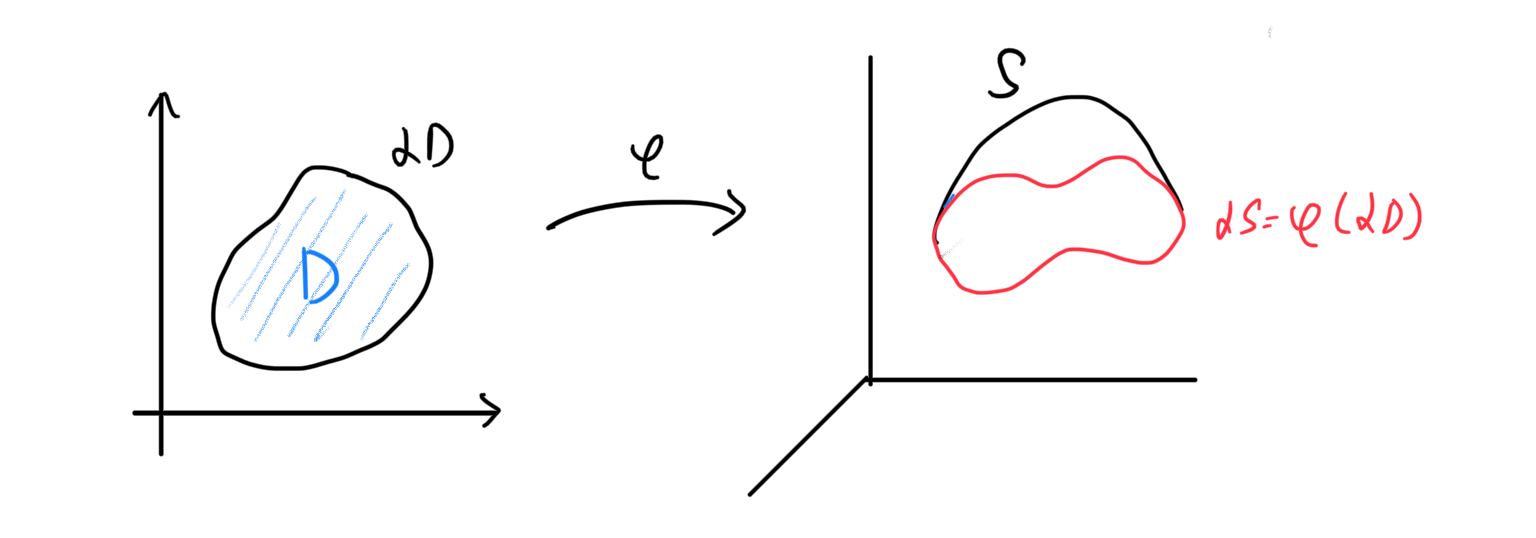
\includegraphics[scale=0.27]{img/Boundary_Mapping.PNG}
  \end{center}
  The orientation unit vector $n$ of $S$ induces the positive orientation of $\partial S$, denoted $\partial S^+$. Visually, if you are walking along the curve with your head is pointing in the same direction as the unit normal vectors while the surface is on the left then you are walking in the positive direction on $\partial S$. 
  \begin{center}
      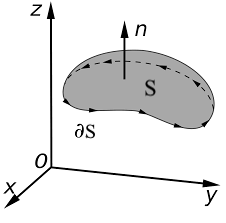
\includegraphics[scale=0.8]{img/Stokes_Theorem_Orientation.png}
  \end{center}
  Given that $F$ is a $C^1$ vector field defined on $S$, then
  \[\iint_S \curl{F} \cdot dS = \iint_S \big( \nabla \times F \big) \cdot d S = \oint_{\partial S^+} F \cdot d s\]
  If $S$ has no boundary, that is, if the image of $p^\prime = \partial S$ is not a simple closed curve, then the integral is $0$. 
  \end{theorem}

  The above theorem implies that the vector surface integral of a surface without a boundary (i.e. a closed graph, such as a sphere) is always $0$ along the curl of any $C^1$ field. Geometrically, this means that given a closed solid $S$ with field $\nabla \times F$, the rate of flow of the vector field into $S$ is equal to the flow out of $S$. 

  \subsubsection{Gauss' Theorem}
  The divergence theorem relates the flux of a vector field through a closed surface to the divergence of the field in the volume enclosed. 

  \begin{theorem}[Gauss' Divergence Theorem]
  Let $V$ be a subset of $\mathbb{R}^3$. Denote by $\partial V$ the oriented closed surface that bounds $V$ (with outward pointing normal orientation vectors), and let $F$ be a $C^1$ vector field defined on a neighborhood of $V$. Then, 
  \[\iiint_V \Div{F} \; d V = \iiint_V (\nabla \cdot F) \; d V = \oiint_{\partial V} F \cdot d S = \oiint_{\partial V} (F \cdot n) \; dS\]
  where the two left-most integrals are volume integrals, and the two right-most integrals are surface integrals. Intuitively, this makes sense; the volume integrals represent the total of the sources in volume $V$, and the right hand side represents the total flow across the boundary $\partial V$. 
  \begin{center}
      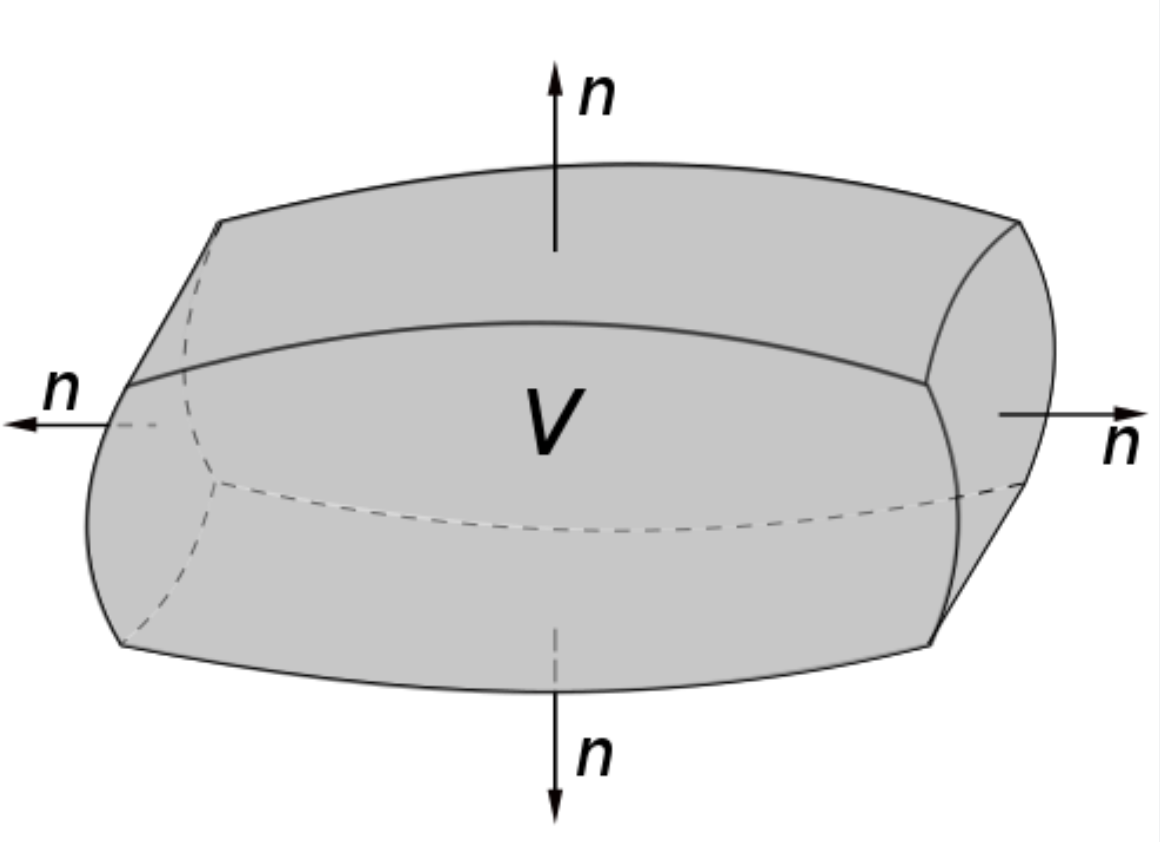
\includegraphics[scale=0.35]{img/Gauss_Theorem_Volume.png}
  \end{center}
  \end{theorem}

\section{Sequences of Functions}



\end{document}
